\chapter{TPC Electronics}
\label{ch:fddp-tpc-elec}


%%%%%%%%%%%%%%%%%%%%%%%%%%%%%%%%%%%%%%%%%%%%%%%%%%%%%%%%%%%%%%%%%%%%
\section{TPC Electronics System Overview}
\label{sec:fddp-tpc-elec-ov}

%%%%%%%%%%%%%%%%%%%%%%%%%%%%%%%%%
\subsection{Introduction}
\label{sec:fddp-tpc-elec-intro}

The aim of the DP TPC electronics is to collect and digitize the signals from the Charge Readout Plane (CRP) and photon detectors, Photo-Multiplier Tubes (PMT), in the Dual-Phase (DP) detector module. The design of the system relies on the components already developed for the ProtoDUNE-DP detector as a result of an R\&D activity started in 2006. One of the key objectives of this R\&D program has been the design of the electronics system that is easily scalable, and cost-effective in order to meet the needs of the large-scale neutrino liquid argon detectors.  

While a single DP detector module has a factor of \num{20} more readout (both charge and light) channels than ProtoDUNE-DP, a simple scaling of the number of the components used in the prototype is sufficient to meet the overall system requirements. A small-scale version of the TPC electronics system has been used in a dual-phase LAr TPC prototype, LArProto, at CERN with an active volume (CRP area) of $3\times 1 \times 1$ \si{\meter\cubed} ($3\times1$ \si{\meter\squared}) that took data in the Summer-Fall 2016. The experience gained from the LArProto operation allowed to validate already some of the design choices and check various performance markers (e.g., noise). 

The Charge ReadOut (CRO) system is designed to provide continuous, non-zero-suppressed, and losslessly compressed digital signals by reading the charge collected on the \SI{3}{m} long strips arranged in two collection views with a pitch of \SI{3.125}{mm} in the CRP. The system consists of a Front-End (FE) analog electronics operating at cryogenic temperatures and digital electronics working in the warm environment outside of the cryostat.  The cryogenic FE analog electronics is based on an ASIC chip with a large dynamic range (up to \SI{1200}{fC}) to cope with the charge amplification in CRP. The analog FE cards are housed in dedicated Signal FeedThrough (SFT) chimneys and are accessible from the outside even after the detector module is in operation thus removing any significant risks associated with their long-term survivability. The SFT chimneys are approximately \SI{2}{m} long objects that traverse the entire insulation layer of the cryostat allowing to place the FE electronics close to the CRP to minimize cable capacitance (noise).  In addition, their metallic structure shield the FE cards from any interference from the digital electronics and ambient environment. The analog signals are digitized by Advanced Mezzanine Cards (AMC), which are housed in the commercial uTCA crates on top of the cryostat near the SFT chimneys. The data are sampled at the rate of \SI{2.5}{MHz} with \SI{12}{bit} resolution.  This frequency, traditionally used in LAr TPC experiments, matches well the \SI{1}{\micro\second} pulse-shaping time of FE electronics and the detector response times determined by the electron drift velocity in the liquid argon. The corresponding sampling resolution along the drift coordinate is better than \SI{1}{\mm}. 

The Light ReadOut (LRO) electronics collects and digitizes the signals from the photon-detector system, which consists of TPB-coated \num{8} inch photomultiplier tubes (Hamamatsu R5912-02-mod) located under the TPC cathode. The LRO electronics should facilitate the detection of the primary scintillation signals, which provide the absolute time reference for the interaction events. It should also enable recording the light signals generated by photons from so-called proportional scintillation component, the light created by the electrons extracted and amplified in the gaseous phase. The electronics, consisting of analog and digital stages, is housed in the uTCA crates on top of the cryostat structure.

Each uTCA crate for either charge or light readout is connected to the DAQ system via an optical fiber link, which support the speed of at least \SI{10}{Gbit/s}. Every crate also contains a module (WR-MCH) for the time synchronization of the digital electronics. This timing slave unit is connected via \SI{1}{Gbit/s} optical fiber to a master node that serves as a synchronization reference for all the connected slave nodes on the network. This system for the time synchronization is based on the commercially available components developed within the framework of the White Rabbit (WR) project. The system performs automatic and continuous self-calibrations to account for any propagation delays and is able to provide sub-ns accuracy for the timing synchronization.


%%%%%%%%%%%%%%%%%%%%%%%%%%%%%%%%%%%%%
\subsection{Design Considerations}
\label{sec:fddp-tpc-elec-des-consid}

The design of the electronics for the charge readout covers the analog front-end cards containing pre-amplifier ASICs operating at cryogenic temperatures and digitization cards with the relevant system for their synchronization working in the warm environment outside of the cryostat. The principle requirements for the system is to read and digitize signals from a total of \num{153600} channels (per one DP detector module) and be capable of continuously streaming the collected and losslessly compressed data to DAQ without any zero suppression. Given the amplification of the ionization charge in CRP, the electronics needs to be sensitive to the signals over a large dynamic range (up-to \num{40} times the MIP-level signals for a nominal CRP gain of \num{20}) to avoid saturation of the analog inputs by large localized energy disposition produced, for example, in hadronic shower events. The charge amplification provided by the CRP loosens requirements on the intrinsic noise of the FE analog electronics. For the CRP nominal gain of \num{20}, the signal-to-noise ratio for a MIP signal (\SI{30}{fC}) should be at least around \num{100}, which would not pose any problems for the detection/reconstruction. The magnitude of noise, however, plays a role in the quality of the lossless compression on the raw data performed by the digital electronics. A compression factor of \num{10} can be achieved with the noise levels below \num{1} ADC RMS.  %be careful of RMS<1...

The primary objective of the light readout system is to detect signals, from a minimum of one photo-electron on one PMT, giving a precise timestamp that can be used in conjunction with the charge signals to determine the time (drift) co-ordinate of an event.  Precise measurements of signal charge will allow the continual monitoring of the PMT gain at the single photo-electron level, and the determination of the number of photons in each scintillation event.  In addition, an ADC will continuously stream data, downsampled to \SI{400}{ns} as for the CRO signals,  which, amongst other items, will allow measurements of the scintillation time-profile. In addition, the light readout system will sample a small number of signals from the PhotoDetection calibration system: the calibration trigger and around \num{20} channels from reference sensors.

The cryogenic analog electronics for charge readout is housed in dedicated SFT chimneys. Their design must enable access to the FE card for possible replacement without any risk of contaminating the pure liquid argon in the main cryostat volume. The chimneys must possess a cooling system that would permit to control the temperature around the FE cards around \SI{110}{\kelvin} for their optimal noise. In addition, the cooling system is to compensate for the heat input from the chimneys into the cryostat volume.

The digital electronics for both charge and light readout is located in the warm environment on the top of the cryostat supporting structure and is therefore easily accessible. This fact removes any constraints associated with the accessibility and operation in cryogenic environments allowing for the usage of standard components and industrial solutions in the design. Digital electronics must be continuously and automatically synchronized to better than \SI{400}{ns} to ensure the correct temporal alignment of the ADC samples from all of the readout channels. This is a minimal requirement dictated by the fact that the sampling rate is \SI{2.5}{\MHz}.  

\begin{dunetable}
[Parameters for the TPC electronics system design]
{lr}
{tab:dpele-physicsparams}
{Parameters for the  TPC electronics system design. The numbers are given for one detector module.}   
Parameter & Value  \\ \toprowrule
  CRO channels    &  \num{153600}            \\ \colhline
  CRO continuous sampling rate & \SI{2.5}{\MHz}\\ \colhline
  CRO ADC resolution & \num{12} bit           \\ \colhline
  CRO data compression factor   & \num{10}    \\ \colhline 
  CRO data flow  & \num{430} Gbit/s          \\ \colhline 
  LRO channels       & \num{720}               \\ \colhline
  LRO continuous sampling rate & \SI{2.5}{\MHz} \\ \colhline
  LRO ADC resolution & \num{14} bit            \\ \colhline
  LRO data compression factor  & \num{1}       \\ \colhline
  LRO data flow   & \num{24} Gbit/s          \\ \colhline
\end{dunetable}

Some of the key parameters in the electronics system design are summarized in Table~\ref{tab:dpele-physicsparams}. The requirements for the DP electronics system are documented in DUNE-docdb-6428.


%%%%%%%%%%%%%%%%%%%%%%%%%%%%%%%%
\subsection{Scope}
\label{sec:fddp-tpc-elec-scope}

The scope of the TPC electronics system covers the procurement and productions, testing and validation, installation, and commissioning of all the components necessary to ensure the complete readout of the charge and light signals from a given DP detector module. The covered items are the following:
\begin{itemize}
\item{Cryogenic analog FE cards for charge readout}
\item{AMC cards for charge/light readout}
\item{The WR-MCH cards for AMC clock synchronization}
\item{uTCA crates}
\item{Switches for the White Rabbit network}
\item{SFT chimneys}
\item{Low-voltage power supplies for the FE cards}
\item{Flat cables connecting the FE cards to the warm flange interface of the SFT chimneys}
\item{VHDCI cables connecting the warm flange interface of the SFT chimneys to AMCs}
\end{itemize}

The total numbers for components to be procured to instrument one detector module are given in Table~ref{tab:dpele-num-components}

\begin{dunetable}
[Numbers for DP electronics components to procure]
{lr} {tab:dpele-num-components}
{Numbers for DP electronics components to procure for one detector module}
Name & Number  \\ \toprowrule
CRO cryogenic ASICs (\num{16} ch) & \num{9600} \\ \colhline
CRO cryogenic analog FE cards (\num{64} ch) & \num{2400} \\ \colhline
CRO AMCs & \num{2400} \\ \colhline
SFT chimneys & \num{240} \\ \colhline
Flat cables for SFT chimney (\num{68} ch) & \num{2400} \\ \colhline
Flat cables for SFT chimney (\num{80} ch) & \num{2400} \\ \colhline
VHDCI cables (\num{32} ch) & \num{4800} \\ \colhline
LRO AMCs with analog FE & \num{45} \\ \colhline
uTCA crates & \num{245} \\ \colhline
WR-MCH units & \num{245} \\ \colhline
WR switches (\num{18} ports) & \num{16} \\ \colhline
\end{dunetable}


%%%%%%%%%%%%%%%%%%%%%%%%%%%%%%%%%%%%%%%%%%%%%%%%%%%%%%%%%%%%%%%%%%%%
\section{TPC Electronics System Design}
\label{sec:fddp-tpc-elec-design}

The CRO FE analog electronics is based on cryogenic ASIC chip with a large dynamic range (up to \SI{1200}{\femto\coulomb}) to accomodate the charge amplification in the dual-phase CRP. The FE cards read \num{64} CRP channels each. They are mounted in dedicated Signal FeedThrough (SFT) chimneys and are located within a short distance (\SI{<1}{\metre}) from each CRP to minimize the noise caused by long cables (large cable capacitance). The cards remain accessible throughout the detector operation. Each SFT chimney hosts \num{10} FE analog cards, which corresponds to the readout of \num{640} CRP channels per chimney. There are, therefore, \num{240} SFT chimneys to be installed for the charge readout in a given DP detector module.   

The differential analog signals from the analog FE cards, routed via an interface flange of the SFT chimneys, are digitized by AMC cards located in the warm conditions outside of the cryostat. AMCs are hosted in uTCA crates. In the baseline version of the design (utilized currently in ProtoDUNE-DP), each AMC digitizes \num{64} channels corresponding to reading one FE analog card. Each uTCA in such case contains \num{10} AMCs (\num{640} channel). However, an implementation with AMCs supporting a higher channel density is also being investigated for cost reduction purposes. A given SFT chimney is serviced by one uTCA crate placed in its immediate vicinity.

The LRO FE analog and digital electronics is based on a custom-built AMC. The card contains a CATIROC ASIC, which is used to determine precisely the charge and start times of signals from each individual PMT. In addition, a \SI{14}{bit} \SI{65}{MHz} ADC digitizes the data for continuous streaming of the PMT signals. Each card can read up to \num{16} channels. A potential future upgrade is to increase the channel density per card to \num{32} channels. The LRO cards are housed in five dedicated uTCA crates located close to the PMT instrumentation feedthroughs.

\begin{dunefigure}[Top view of DP detector module]{fig:dpele-sft-chimney-pattern}
{Corner view of DP detector module showing the pattern of the SFT chimneys and uTCA crates for charge readout above CRPs}
\includegraphics[width=0.6\textwidth]{dpele-sft-chimney-pattern}
\end{dunefigure}

Every uTCA crates contains a network switch, MicroTCA Carrier Hub (MCH), via which the data are sent to DAQ as well as a module (WR-MCH) for clock/time synchronization and trigger timestamp distribution to the AMCs. Both MCH and WR-MCH require one optical fiber link each. 

The MCH switch streams the data from AMCs via a dedicated optical link. Currently ProtoDUNE-DP uses MCH operating at \SI{10}{Gbit/s}. However, a move to \SI{40}{Gbit/s} links for the DUNE FD implementation is considered because of the technology evolution and possible increase in the channel density of each AMC.

The WR-MCH time synchronization unit is based White Rabbit (WR) system, which provides hardware and protocols for the network-based sub-ns synchronization between a master and different slave nodes. The connection of the WR-MCH to the White Rabbit network is done via \SI{1}{Gbit/s} optical link. WR-MCH distributes the timing information for synchronization of the AMCs via the uTCA backplane. In addition, this unit can be used to transmit triggers to the digitization units within the crate. This is achieved by sending it dedicated data packets containing trigger timestamp information. 

Figure~\ref{fig:dpele-sft-chimney-pattern} shows a corner view of the DP detector module illustrating the pattern of the SFT chimneys and the attached uTCA crates above the CRPs. Each crate/SFT chimney collects signals from \SI{3}{\meter} long strips of two \SI[product-units=power]{1x3}{\meter} CRP segments. Each chimney completely traverses the insulation layers (not shown in the figure). 
%A cut-out view of the chimney illustrates the location of the FE cards and provides the overall scale of this object. 


\begin{dunetable}
[Summary of some of the principal numbers of the TPC electronics system.]
{lr} {tab:dpele-numparts}
{Summary of some of the principal numbers of the TPC electronics system for charge and light readout of a detector module}
Name & Number  \\ \toprowrule
   CRO SFT chimneys/uTCA crates              &  \num{240}   \\ \colhline
   CRO channels per SFT chimney/uTCA crate & \num{640} \\ \colhline
   CRO cryogenic analog FE cards per SFT chimney    &  \num{10}     \\ \colhline
%   CRO Cryogenic analog FE cards (total)                   & \num{2400}  \\ \colhline
   CRO AMCs per uTCA crate                       & \num{10}      \\ \colhline
%   Charge readout AMCs (total)                                   & \num{2400}      \\ \colhline 
   LRO FE cards  per uTCA crate & \num{9} \\ \colhline
%   Light readout FE cards (total)           & \num{45} \\ \colhline
   LRO channels per uTCA crate & \num{144} \\ \colhline
   LRO uTCA crate                      & \num{5} \\ \colhline
   WR-MCH per uTCA crate                 & \num{1} \\ \colhline
%   WR-MCH (total)                              & \num{245} \\ \colhline
%   uTCA crates (total)                         & \num{245} \\ \colhline
\end{dunetable}

A short summary of some of  the number of principal components and channel granularity in the design of the DP electronics is provided in Table~\ref{tab:dpele-numparts}. 

%%%%%%%%%%%%%%%%%%%%%%%%%%%%%%%%%%%
\subsection{Cryogenic Analog FE Electronics}
\label{sec:fddp-tpc-elec-design-cryofe}

The cryogenic amplifer ASIC is the main component of the FE analog cards. Its design is based on the CMOS \SI{0.35}{\micro\meter} technology and is an outcome of an R\&D  activity started in 2006. Two principal version of ASIC chips have been produced for the dual-phase LArTPC operation. In the first version the amplifiers have a constant gain in the region of $0-1200$ \si{\femto\coulomb} ($0-40$ MIP). In the second, the amplifiers have a higher linear gain for signals up to \SI{400}{\femto\coulomb} (roughly 10 MIP signals) and a logarithmic response in the  $400-1200$ \si{\femto\coulomb} range. This double-slope behavior is obtained by using a MOSCAP capacitor in the feedback loop of the amplifier that changes its capacitance above a certain signal threshold. The aim of this solution is to optimize the resolution for small charge depositions (in a few MIP region) while preserving overall the large dynamic range of the amplifier.

\todo{update figure with only two curves for -162 and 27 C}
\begin{dunefigure}[Gain response of the cryogenic FE ASIC]{fig:dpele-fe-asic-gain}
{Gain response of the cryogenic FE ASIC }
%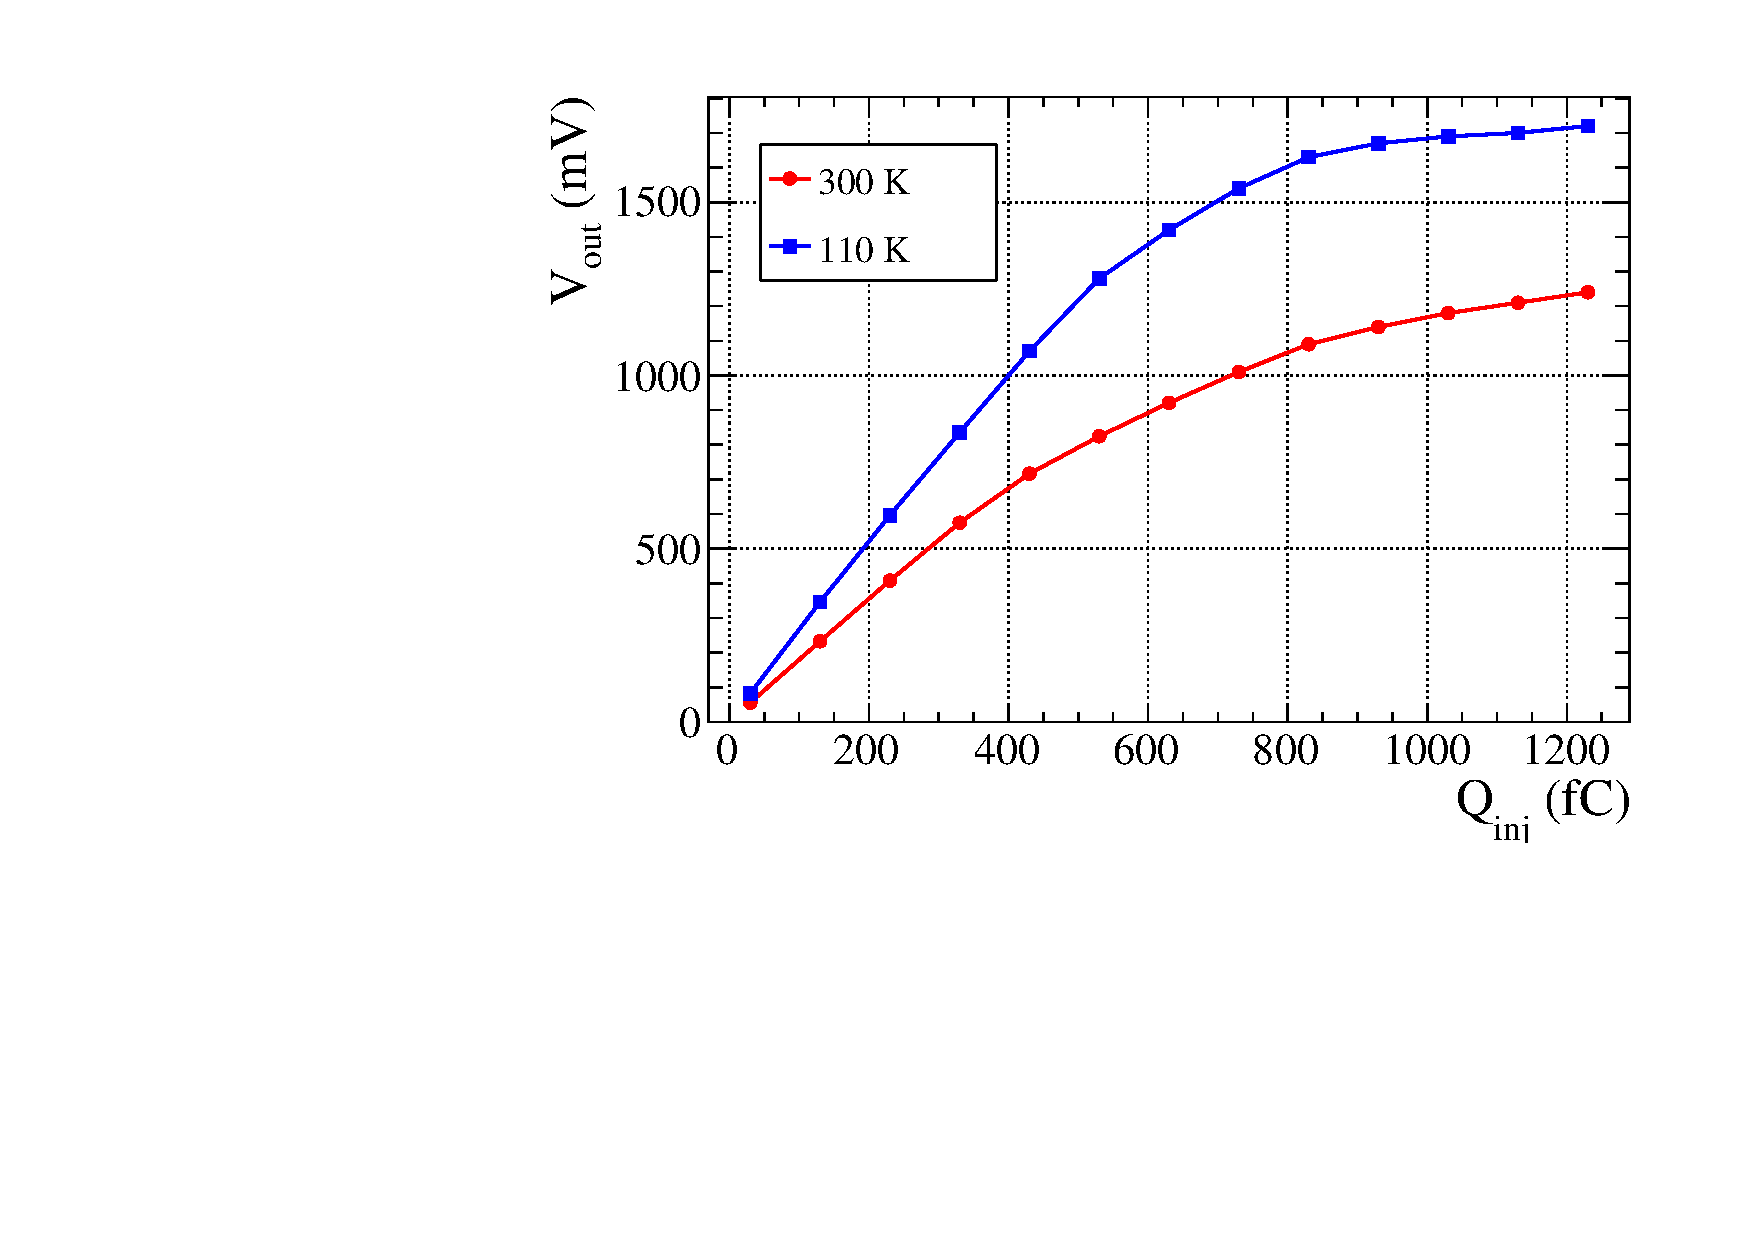
\includegraphics[width=0.5\textwidth]{dpele-fe-asic-gain}
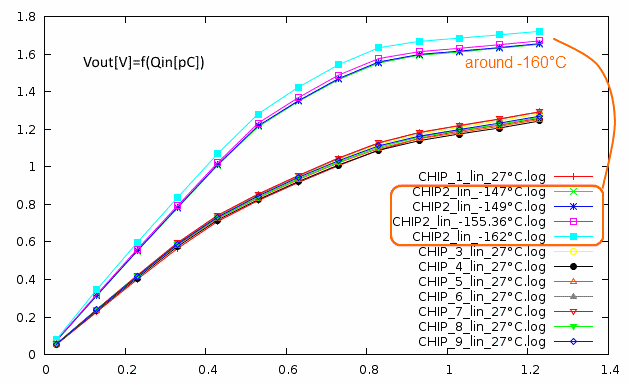
\includegraphics[width=0.5\textwidth]{larzic_2015_slope}
\end{dunefigure}

\todo{update figure with  only two curves for -162 and 27 C}
\begin{dunefigure}[Noise of the cryogenic FE ASIC as a function the detector capacitance]{fig:dpele-fe-asic-noise}
{Noise of the cryogenic FE ASIC as a function the detector capacitance}
%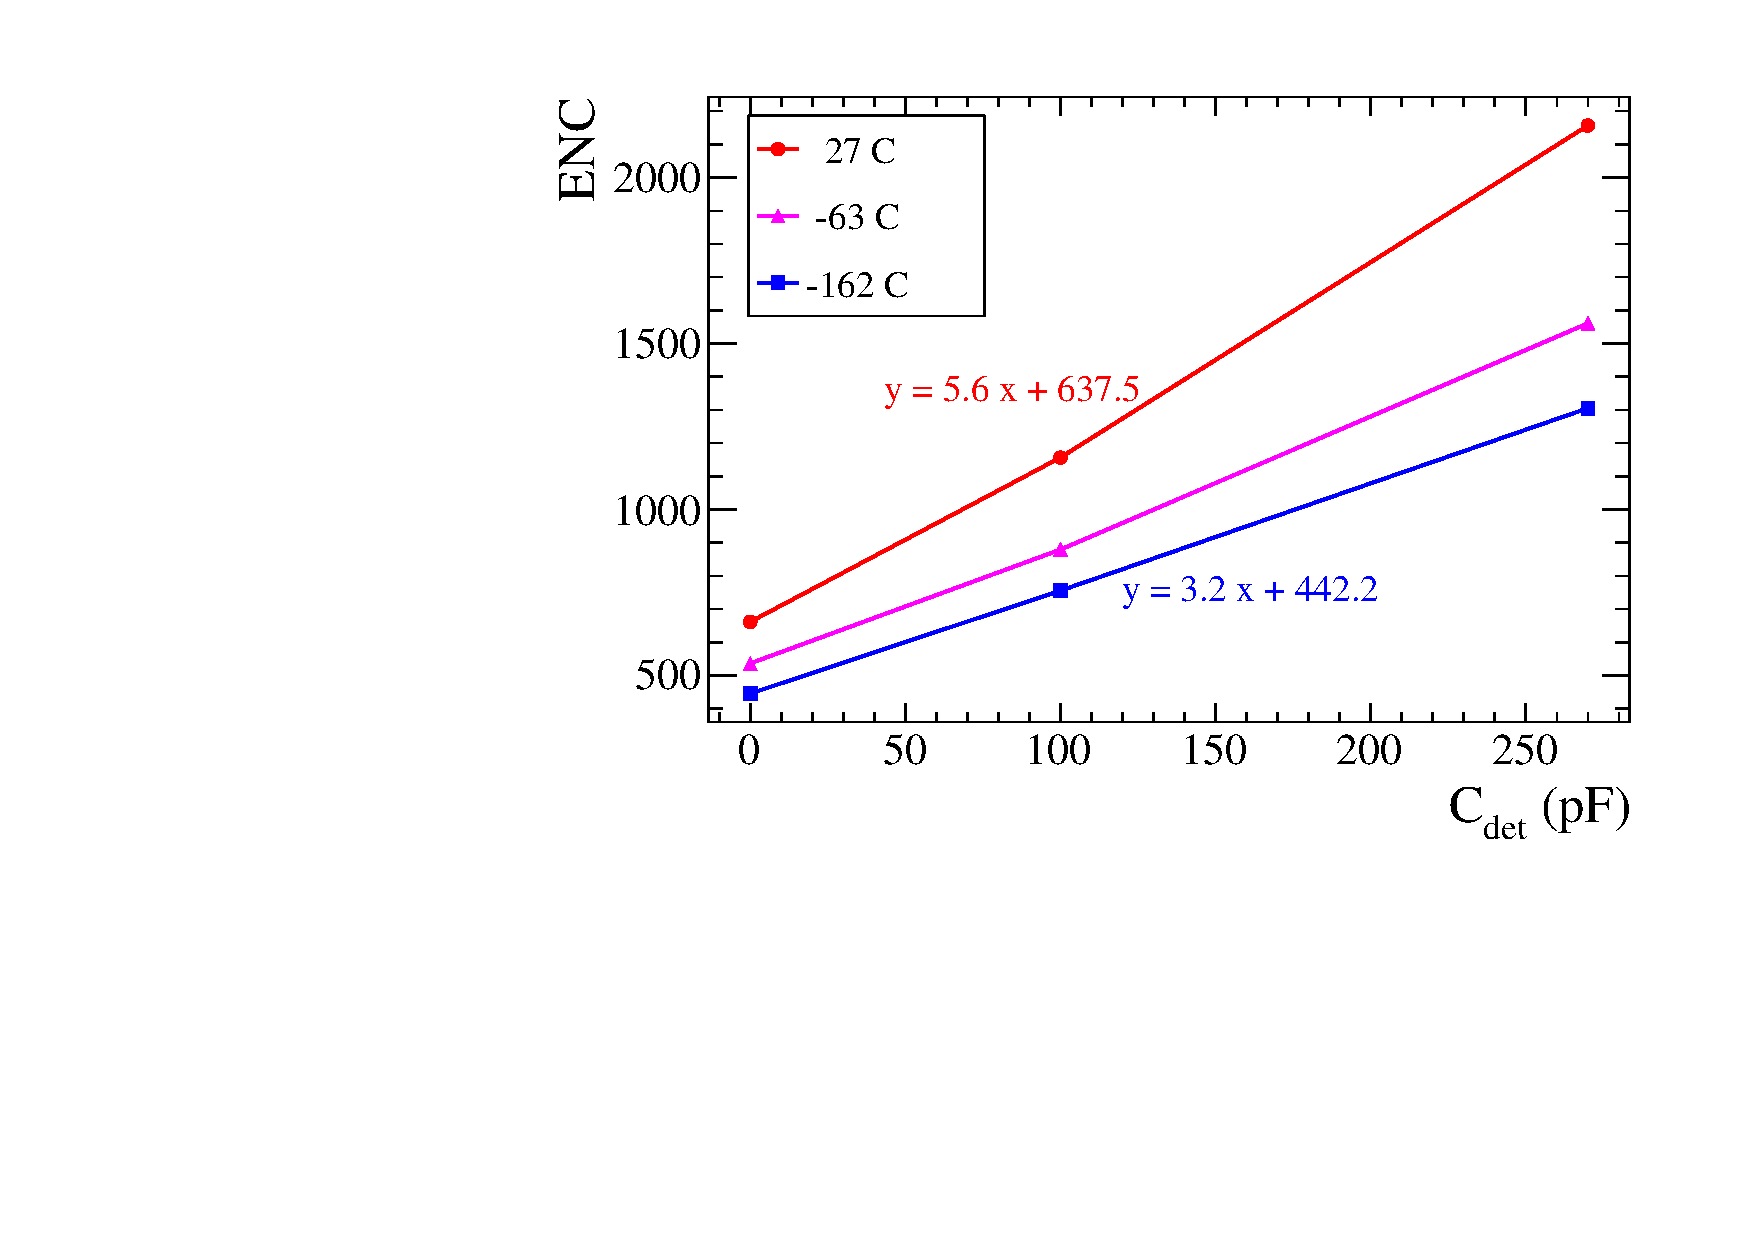
\includegraphics[width=0.5\textwidth]{dpele-fe-asic-noise}
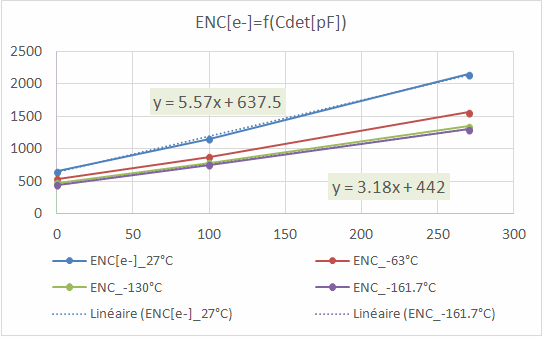
\includegraphics[width=0.5\textwidth]{enc_cdet}
\end{dunefigure}

The ASIC version with the double-slope gain has been selected for ProtoDUNE-DP and adopted in the DP TPC electronics design. Figure~\ref{fig:dpele-fe-asic-gain} illustrates the response of the amplifier as a function of the injected charge for this chip, while Figure~\ref{fig:dpele-fe-asic-noise} shows the measured noise in units of Equivalent Noise Charge (ENC) as a function of the ("detector")  capacitance at different temperatures. The ASIC contains \num{16} amplifier channels with differential line buffers and has a power consumption which is \SI{<18}{\milli\watt} per channel. 

\begin{dunefigure}[Image of an analog FE card mounted on the extraction blade]{fig:dpele-fe-card-blade-image}
{Image of an analog cryogenic FE card mounted on the extraction blade}
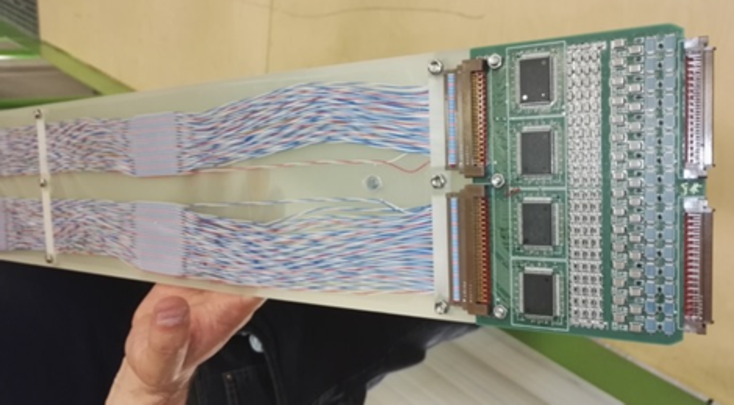
\includegraphics[width=0.7\textwidth]{dpele-fe-card-blade-image}
\end{dunefigure}

Each cryogenic FE card, shown in Figure~\ref{fig:dpele-fe-card-blade-image}, hosts four ASIC amplifier chips and a few passive discrete components. The input stage of each amplifier channel has a \SI{1}{\giga\ohm} resistor to ground followed by a \SI{2.2}{\nano\farad} decoupling capacitor. The function of the resistor is to provide the ground reference for the anode strips of CRP. Each input stage is protected against discharges coming from the detector with a TVS diode (Bourns CDSOD323-T08LC). This component was selected after studying the performance of different ESD components subjected systematically to discharges of a few kV with an energy similar to that of LEMs in CRP. The FE cards also house the blocking capacitors for filtering the low voltage power lines.

\begin{dunefigure}[Noise measurements in LArProto in different conditions]{fig:dpele-311-noise}
{Noise of measurements in LArProto in different conditions. Left: at warm with the slow control cables connected to the cryostat flanges (red points) and disconnected (black points). Right: at warm (red points) and cold (black points) with the slow control cables disconnected. The channels with negative (positive) channel number correspond to the strips of \SI{3}{\meter} (\SI{1}{\meter})}
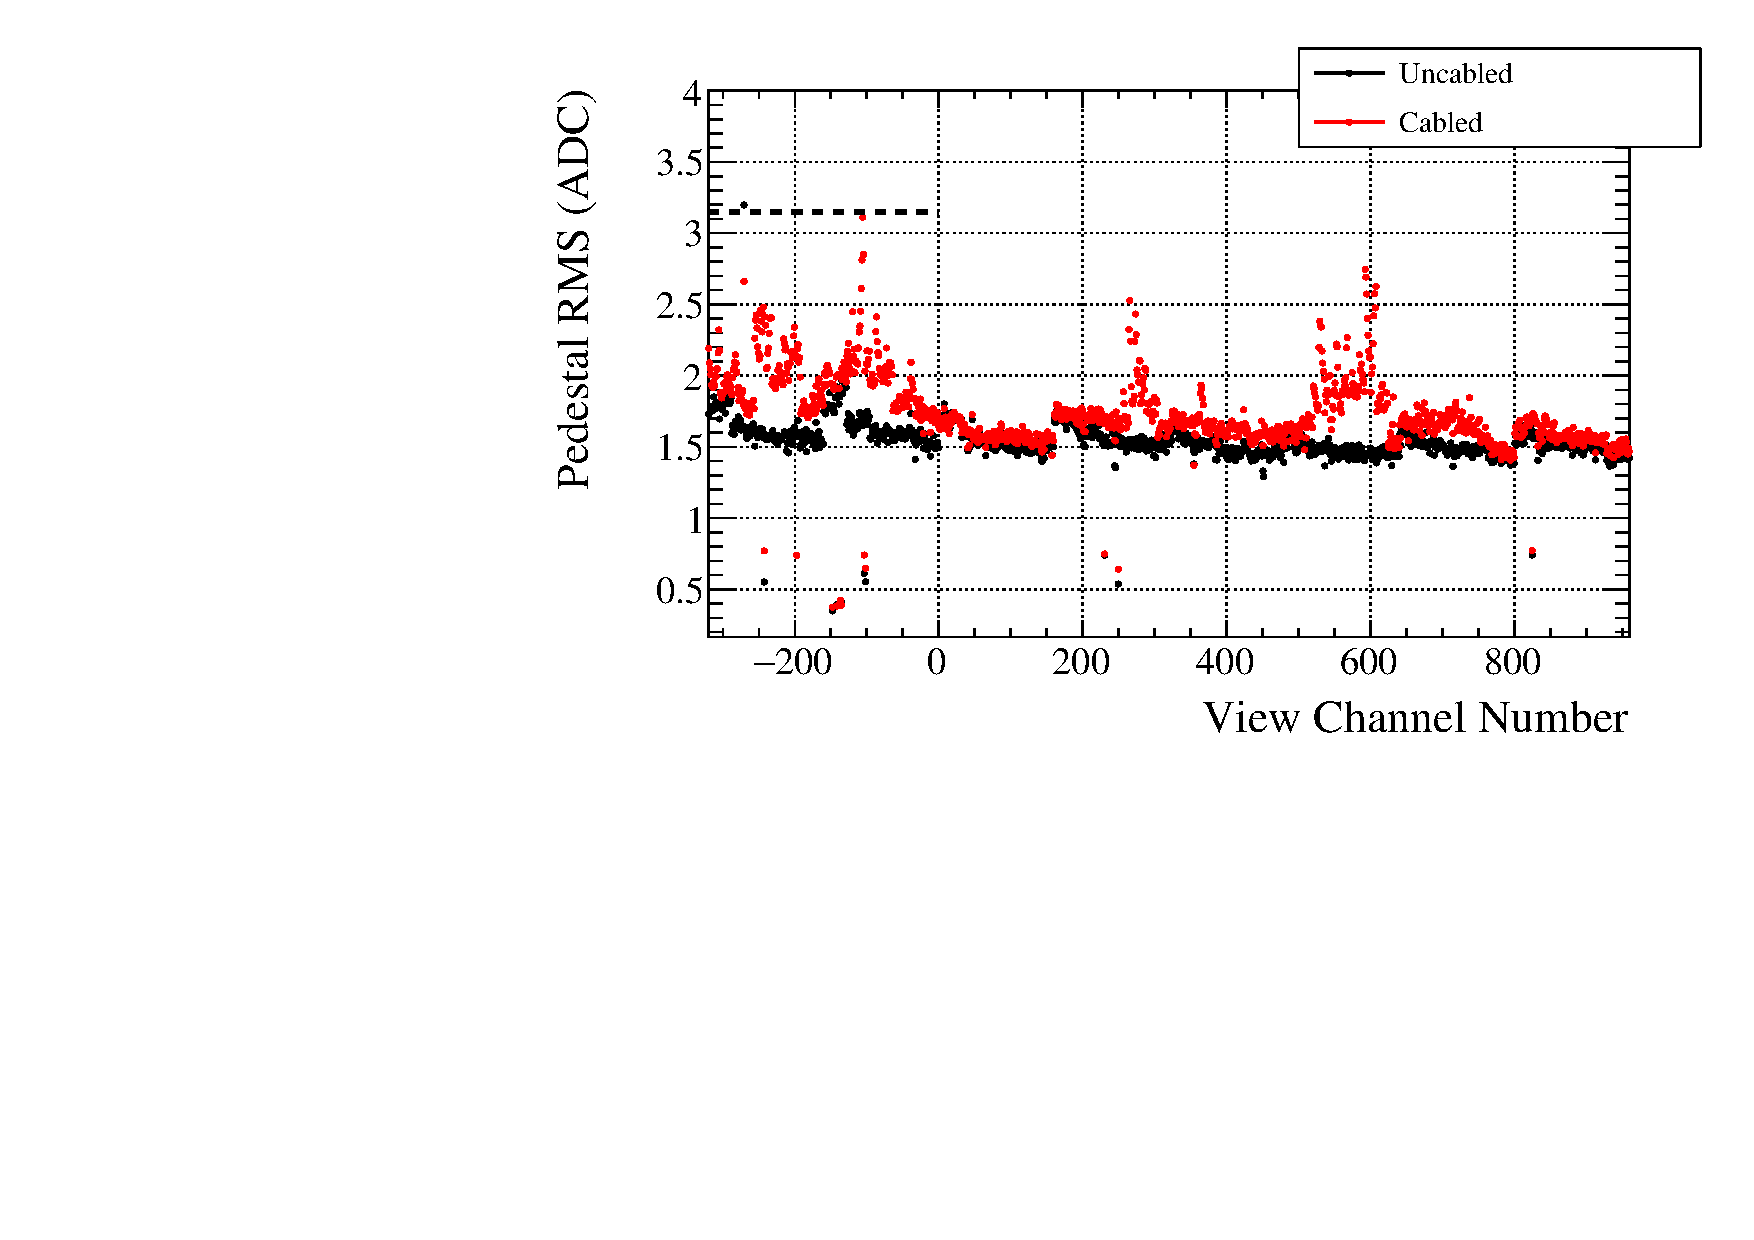
\includegraphics[width=0.45\textwidth]{dpele-311-noise-warm}
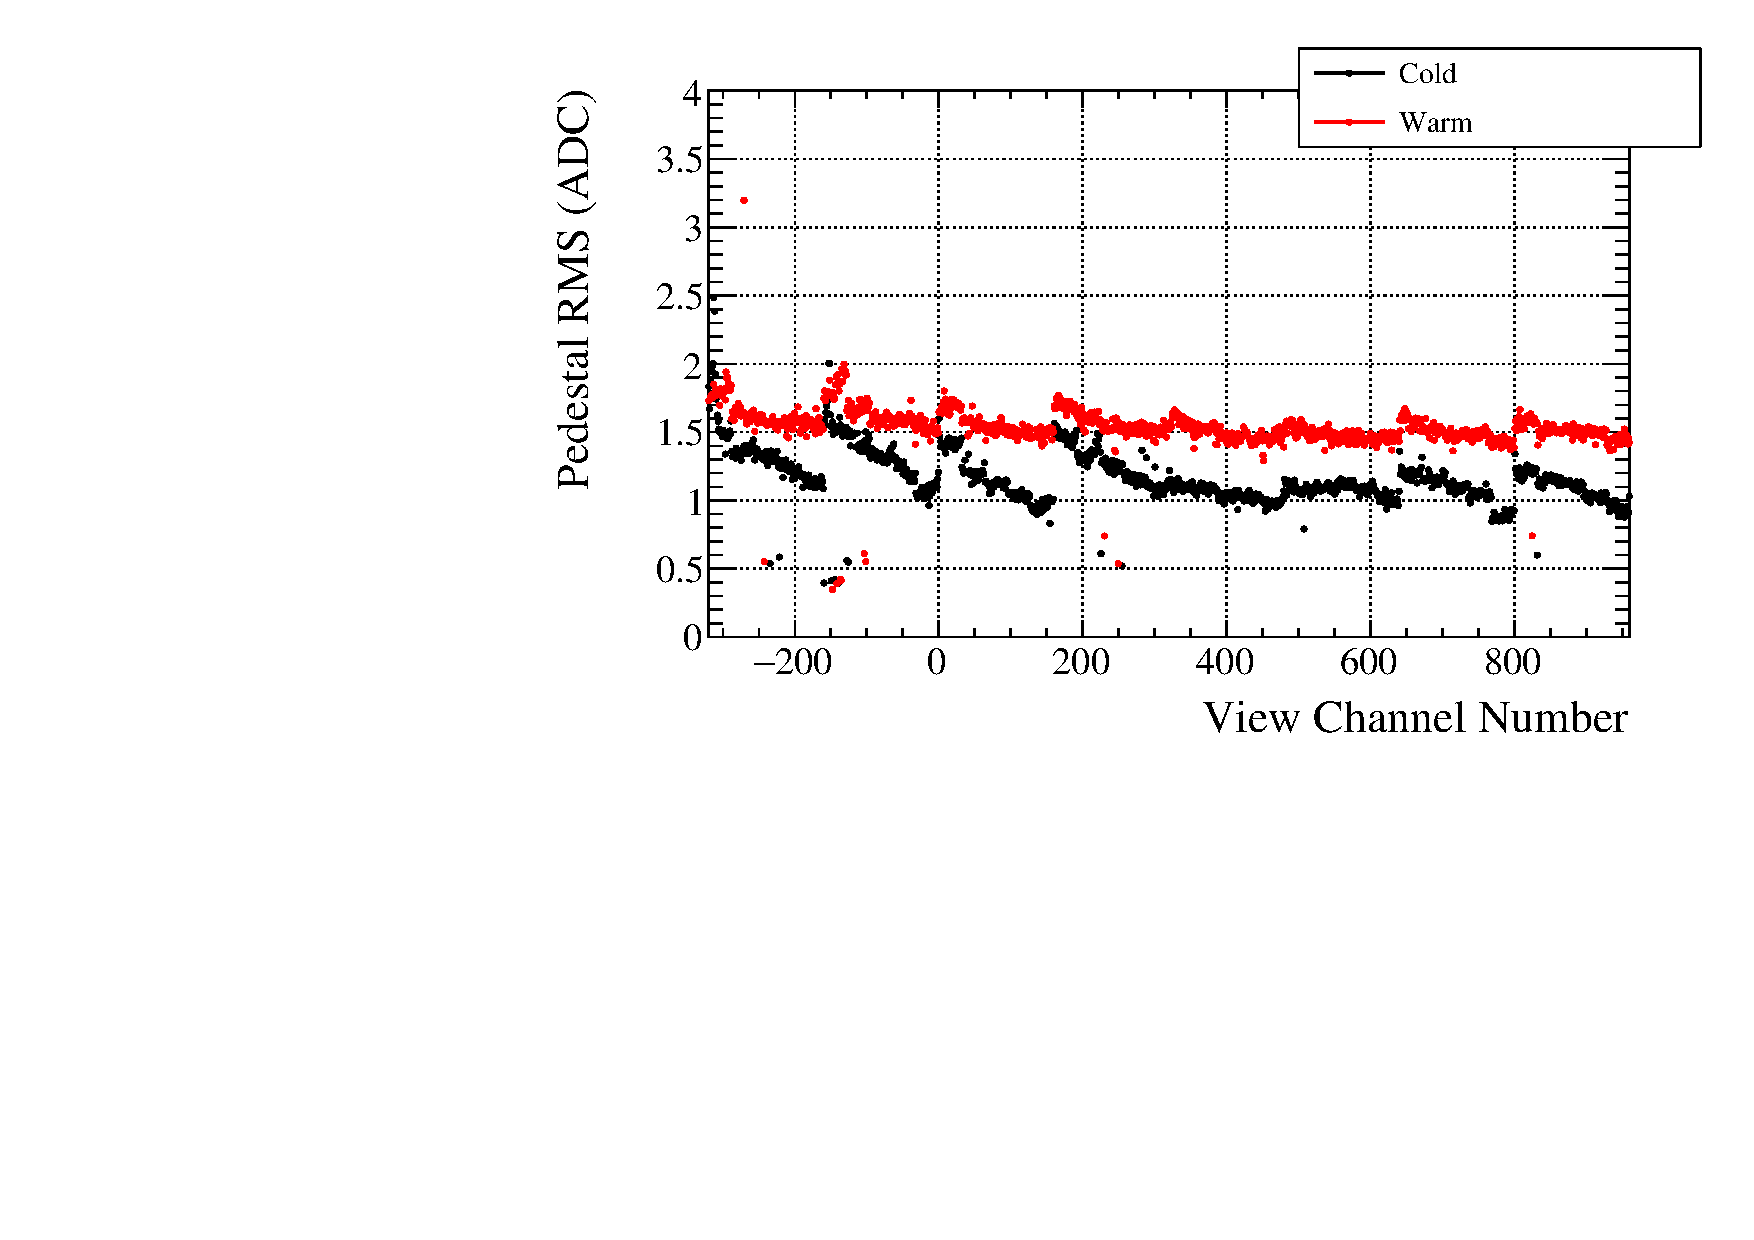
\includegraphics[width=0.45\textwidth]{dpele-311-noise-warm-cold}
\end{dunefigure}

While the FE amplifier ASICs are in the shielded environment provided by the chimneys (Faraday cage), interference from other equipment via a noisy ground or ground loops could significantly worsen the noise performance from the design target. Figure~\ref{fig:dpele-311-noise} shows some results of the noise measurements performed under different conditions in the LArProto detector. The channels reading \SI{3}{\meter} (\SI{1}{\metre}) long strip correspond to negative (positive) channel numbering in the plots and the 1 ADC count is equivalent to about 900 electrons. The left plot of Figure~\ref{fig:dpele-311-noise} shows the noise measurements performed at warm with and without slow control cables (CRP HV, CRP motors, level meters, temperature probes, etc.) connected. The noise is clearly affected by the grounding of the slow control: the average value of the noise RMS is around \num{1.7} ADC with slow control cables connected and decreases to about \num{1.5} ADC when those are removed. One interesting feature, particularly visible with the cables disconnected, is that the noise measured in LArProto is similar for the channels connected to the \SI{1}{\meter} and \SI{3}{\meter} long strips. Given that the longer strips have thrice the input capacitance than the shorter ones, the expected noise (see Figure~\ref{fig:dpele-fe-asic-noise}) for these should be larger by a factor of \num{2} as indicated by the dashed line in the plot. In addition, the noise on the short strips is also lower (\num{1.5} ADC) than expected for the \SI{160}{pF/m} strip input capacitance (1.7 ADC). The reason for such behaviour of the noise in the CRP of LArProto is still under investigation. However, measurements have shown that the capacitance of the CRP anode strips is not purely to ground, but rather it is driven by the inter-strip couplings, which creates a more complicated electrical network. 

Figure~\ref{fig:dpele-311-noise} (right) also shows a comparison of the noise measurements in LArProto taken with the FE electronics at warm (red points) and cold (black points) at around \SI{150}{\kelvin}. The slow control cables were disconnected in both cases. However, the measurements at cold were performed with the re-circulation pump active and the cathode HV connection present. The RMS noise averaged over all channels decreases by about 25\% from roughly \SI{1.5} ADC to \SI{1.1} ADC when the FE analog cards are at cold. For comparison, the expected signal for a MIP with the CRP gain of 20 should be around \num{200} ADC. 

The overall grounding principle of LArProto was based on having the cryostat as the ground reference. The low voltage power supplies for the FE analog electronics and uTCA crates were powered via insulating transformers ensuring that they could see no other ground. On the other hand, the design of the slow control system did not include any insulation transformers. This equipment was the grounded to the building electrical network thereby creating an interference with the ground of the cryostat. Stricter treatment of the ground connections to the detector module  and a lower SFT chimney operating temperature of around \SI{110}{\kelvin} (from \SI{150}{\kelvin}) should help to reduce further the noise levels from those observed in LArProto.


%%%%%%%%%%%%%%%%%%%%%%%%%%%%%%%%%%%
\subsection{SFT Chimneys}
\label{sec:fddp-tpc-elec-design-sft}

The SFT chimneys are designed to enable the access to the FE analog electronics for a potential repair or exchange while the detector is in operation (filled with the liquid argon). In addition, their metallic structure acts as a Faraday cage isolating the FE ASICs from environmental interference.  Each SFT hosts \num{10} analog cryogenic FE cards (reading \num{640} channels in total).  Some of the details of the design are illustrated in Figure~\ref{fig:dpele-sft-chimney-design}. 

\begin{dunefigure}[Details of the SFT chimney design]{fig:dpele-sft-chimney-design}
{Details of the SFT chimney design}
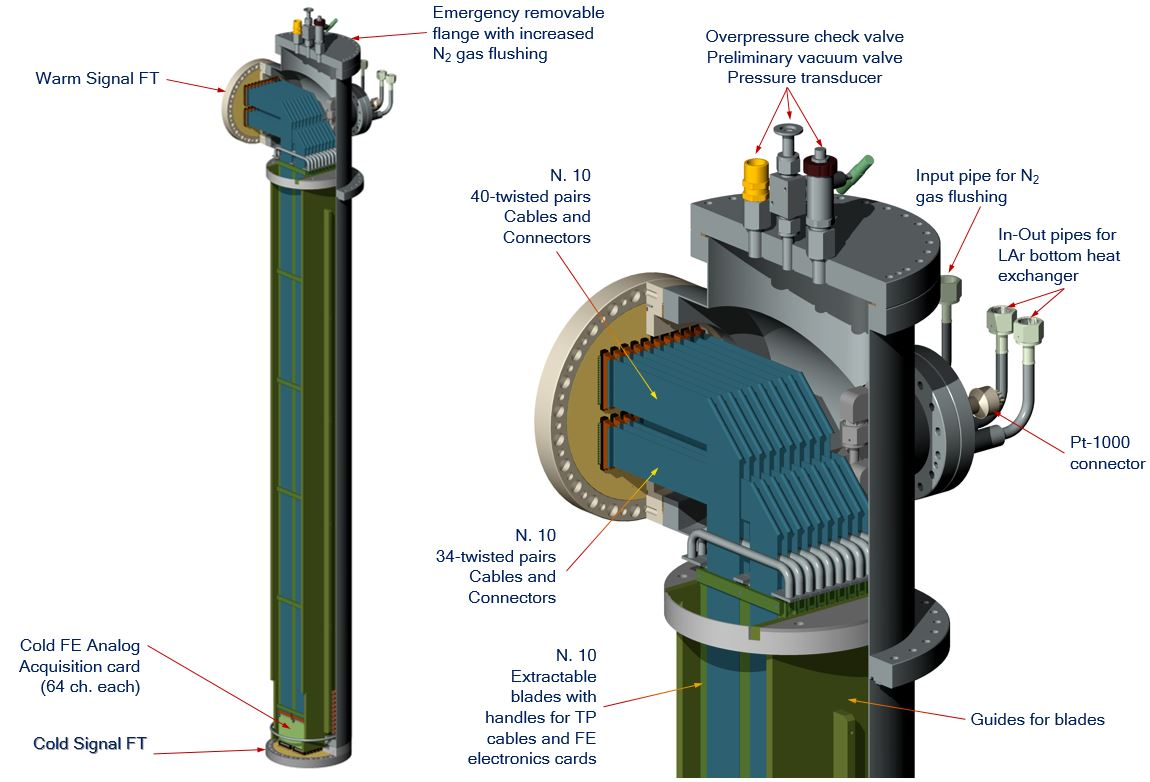
\includegraphics[width=0.8\textwidth]{dpele-sft-chimney-design}
\end{dunefigure}

The chimneys are closed at the bottom and top with vacuum tight flanges whose function is to dispatch the signal and slow control lines. The flange at the bottom, the cold flange, isolates (Ulta-High Vacuum tightness standard) the inner volume of the detector module from the chimney volume and interconnects the signals from the CRP to the analog FE cards. The flange at the top, the warm flange, seals the chimney from the outside environment. It also passes the low voltage and control lines to the FE electronics inside and brings out the differential analog signal lines from the FE amplifiers. 

The SFT chimney volume is filled with nitrogen gas at near atmospheric pressure. The temperature inside the chimney can be adjusted using a heat exchanger copper coil cooled with liquid argon. It is located at the bottom close to the cold flange around the FE cards. The functions of this cooling system are to mitigate the heat input to the main detector volume and provide optimal (lowest noise) operating temperature for the FE electronics of around \SI{110}{K}. A pressure release valve, indicated in Figure~\ref{fig:dpele-sft-chimney-design}, protects the structure from an accidental overpressure in the inner volume. 

The expected heat input from a given SFT chimney is about \SI{20}{\watt}. This number includes the heat through the twisted-pair cables connected to the warm flange, the SFT outer metallic tube, as well as the heat dissipation by the FE cards. A total heat input from all \num{240} SFT chimneys is at the level of \SI{5}{\kilo\watt}. 

\begin{dunefigure}[SFT chimney cold flange]{fig:dpele-sft-cold-pcb}
{SFT chimney cold flange with one of the FE cards mounted }
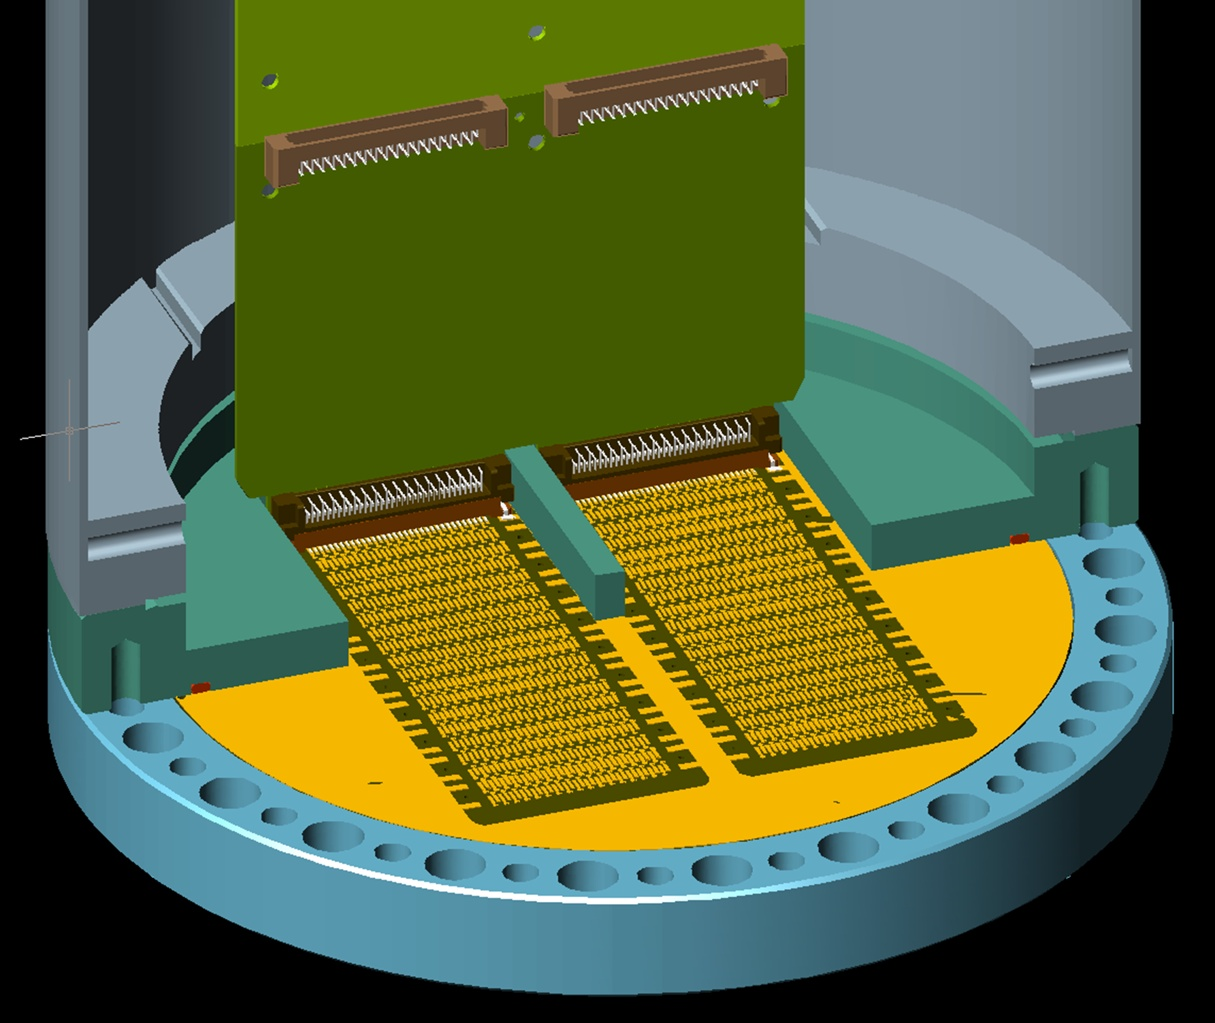
\includegraphics[width=0.6\textwidth]{dpele-sft-cold-pcb}
\end{dunefigure}

The analog FE cards are inserted directly onto the PCB of the cold flange (see Figure~\ref{fig:dpele-sft-cold-pcb}). The other side of the PCB (facing inside the cryostat) hosts the connectors for the flat cables coming from the CRP anodes.  The FE cards are mounted on \SI{2}{m} long blades made from FR4, which enable the insertion/extraction of the electronics and also support the flat cables carrying signals, low voltages, and slow control to/from the warm flange interface.  The blades slide along the rails installed inside the chimney at opposite sides, which guide the FE cards to their respective connectors on the cold flange. 

Prior to the commissioning of a detector module, the chimneys are evacuated via a dedicated KF16 port (see Figure~\ref{fig:dpele-sft-chimney-design}) and then filled with nitrogen gas. This ensures the removal of the moisture that would otherwise condense, once the detector module is filled with the liquid argon, around the FE cards damaging the electronics. To access the FE cards once the detector module is cold, the stainless steel flange at the top of the SFT chimney (Figure~\ref{fig:dpele-sft-chimney-design}) must be removed. This procedure requires continuous flushing of nitrogen gas at slight over-pressure with respect to the atmospheric in order to prevent the humid air entering and generating condensation inside the chimney. Once a chimney is opened, the blades with the FE cards can be extracted after unplugging the flat cables (two per card) connected on the inner side of the warm flange (Figure~\ref{fig:dpele-sft-chimney-design}).

The procedure to access the FE cards at cold was successfully tested during the operation of the LArProto detector. The temperature at the top of the chimney was very close to the room temperature allowing to manipulate the cable connections one warm flange without any cryogenic gloves. The movement of the blades on the rails and the FE card extraction / insertion did not indicate any mechanical problems that could have been caused by shrinking of various elements due to the lower temperatures.  The signals from the FE cards that underwent the extraction/insertion were also checked and no malfunctioning channels were found.

%%%%%%%%%%%%%%%%%%%%%%%%%%%%%%%%%%%
%\subsection{Low-voltage Power Supplies for FE Electronics}
%\label{sec:fddp-tpc-elec-design-lvps}

%%%%%%%%%%%%%%%%%%%%%%%%%%%%%%%%%%%
\subsection{Digital AMC Electronics for Charge Readout}
\label{sec:fddp-tpc-elec-design-amc}
%THIS IS CHARGE READ OUT
The function of the CRO AMC cards is to read and digitize the data from the FE amplifier and then transmit them to the DAQ system. Each card has eight ADC chips (AD9257), two dual-port memories (IDT70T3339), and an FPGA (ALTERA Cyclone V) on board. The FPGA provides a virtual processor (NIOS) that handles the readout and the data transmission.  The cards also include a last stage of analog shaping before the ADC input.

\begin{dunefigure}[Block diagram of AMC]{fig:dpele-amc-scheme}
{Block diagram of AMC}
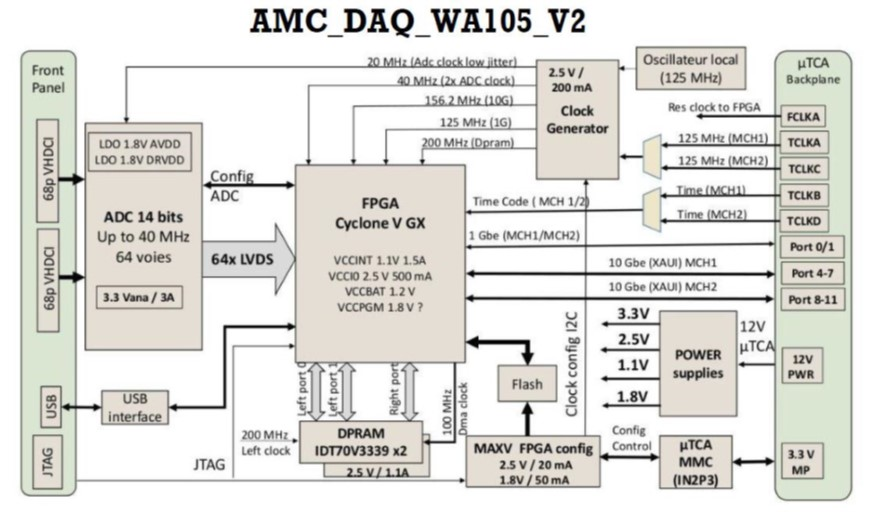
\includegraphics[width=0.7\textwidth]{dpele-amc-scheme}
\end{dunefigure}

Figure~\ref{fig:dpele-amc-scheme} shows block diagram of the AMC functionality. The data are continuously sampled at \SI{2.5}{\MHz} with \num{14} bit resolution. However only \num{12} most significant bits of each sample are eventually sent to the DAQ. Within AMCs lossless data compression based on an optimized version of the Huffman algorithm is performed and the data are organized in frames for transmission. The frames contain the absolute timing information of the first data sample.  In the current design, each AMC has 64 channels and reads one analog FE card.

The AMCs are housed in uTCA crates and send their data via the MCH switch. The timing synchronization of AMCs is achieved via a WR-MCH module (also housed in the crate) that is connected to the White Rabbit network. In addition, WR-MCH could also be used for triggered readout of AMCs by sending it dedicated packets containing trigger timestamp information over the White Rabbit network.

In ProtoDUNE-DP, AMCs are operated in the triggered mode reading \SI{4}{\milli\second} drift time window at trigger rate of \SI{100}{Hz}, which is not far from a continuous readout mode. The analog data are continuously digitized and buffered. A sub-sample of this data can then be acquired by providing AMC with a timestamp generated by an external trigger. The timestamp defines the start time for the data sequence to be read, while the length of the sequence is determined by the size of the drift window. In ProtoDUNE-DP this length corresponds to \num{10000} (\SI{4}{\milli\second}) samples per full drift window.  Triggers (beam counters, cosmic ray counters, photomultipliers reading the UV light, starts of beam spills) are time stamped in a dedicated White Rabbit slave node (WR-TSN), an FMC-DIO mezzanine mounted on WR SPEC carrier card, which runs a custom firmware and is hosted in a computer. The WR-TSN is connected to the WR Grand Master for synchronization and for transmission of the trigger information. The timestamp data produced by the WR-TSN are sent over the White Rabbit network as Ethernet packets with a customized protocol. 

%%%%%%%%%%%%%%%%%%%%%%%%%%%%%%%%%%%
\subsection{Electronics for Light Readout}
\label{sec:fddp-tpc-elec-design-lro}

%
The LRO card is a \num{16} channel AMC containing one \num{16} channel \num{14} bit \SI{65}{\MHz} ADC (AD9249) and one CatiROC ASIC \cite{catiroc}. A block diagram of the prototype board used for ProtoDUNE-DP is shown in Figure~\ref{fig:dpele-lro-scheme}. In this prototype, Figure~\ref{fig:dpele-lro-proto}, a mezzanine board containing the ASIC and ADC sits on a commercial (COTS) mother board (Bittware S4 AMC) with a high specification FPGA (ALTERA Stratix IV). In the final implementation for the DUNE, the mezzanine is integrated with the layout of the AMC board developed for the charge readout.  
A proposed upgrade is a \num{32} channel card, diminishing the number of cards required and increasing the channel density to \num{352} channels per uTCA crate.

\begin{dunefigure}[Block diagram of LRO]{fig:dpele-lro-scheme}
{Block diagram of LRO prototype.}
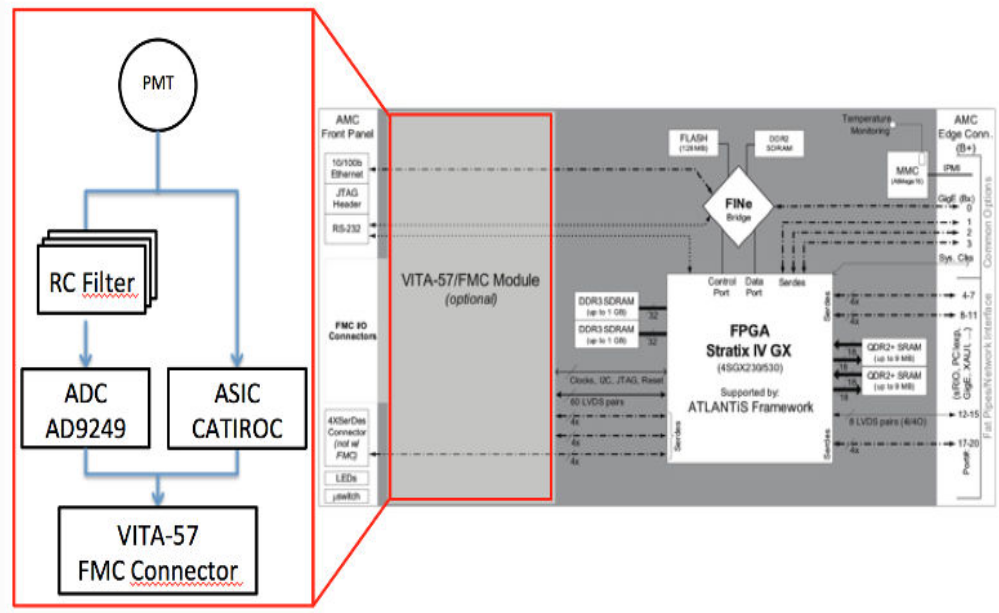
\includegraphics[width=0.7\textwidth]{dpele-lro-scheme}
\end{dunefigure}

\begin{dunefigure}[Prototype LRO card]{fig:dpele-lro-proto}
{The LRO prototype.}
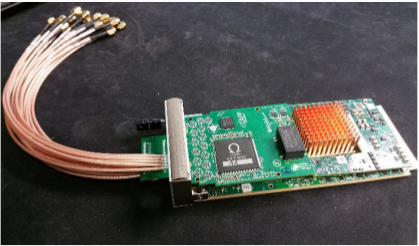
\includegraphics[width=0.7\textwidth]{dpele-lro-proto}
\end{dunefigure}

The analog signals from each PMT channel follow two separate branches (see Figure~\ref{fig:dpele-lro-scheme}) . One path (Waveform branch), through an anti-aliasing low-pass filter and the \num{14} bit \SI{65}{\MHz} ADC (AD9249), produces continuous digitization of the PMT waveform data, which are down-sampled to \SI{2.5}{MHz} prior to the transmission to DAQ. The other (CatiROC branch) is routed directly to the CatiROC ASIC for precise measurements of pulse charge and timing. Both paths produce data continuously and independently.


\subsubsection{Waveform branch} %ADC
%details on CatiROC
The main characteristics of the ADC used for continuous digitization of the PMT signals are shown in Table \ref{tab:dpele-adc}.
%RMS and PMT gain?
\begin{dunetable}
[Main characteristics of ADC AD9249]
{lr} {tab:dpele-adc}
{Main characteristics of the ADC AD9249}
Item &   \\ \toprowrule
Time resolution & \SI{15}{ns} \\ \colhline
Amplitude resolution (LSB) & \SI{0.122}{mV} \\ \colhline
Dynamic range & \num{14} bit/ \SI{2}{V} \\ \colhline
Differential Non-Linearity & Typical $\pm$\num{0.6} LSB\\
& with Min. \num{-0.9} and Max. \num{+1.6} LSB  \\ \colhline
Integral Non-Linearity & Typical $\pm$\num{0.9}  LSB\\
& with Min. \num{-3} and Max. \num{3} LSB  \\ \colhline
%MEMORY??
\end{dunetable}
%noise llevel??

For normal operation, in continuous sampling mode, the time samples will be down-sampled by the FPGA to a coarse \SI{400}{ns} sampling to match that of the Charge Read Out and limit the quantity of data streamed. Before this downsampling, there is the possibility of online pulse processing within the FPGA, to make continuous measurements such as rise and fall times. Even at the coarse sampling of \SI{400}{ns} studies of the liquid argon scintillation time-profile are possible (with the long fall timeconstant of $\sim$\SI{1500}{ns}) and also matching of the electroluminescence signal (also known as proportional scintillation light) to that of the charge signal.  Low light-level signals, such as the single or few photoelectron signals, will show no time structure, but will consist of 1 sample several LSB above the baseline. 

\subsubsection{CatiROC branch} %{Analog Measurements of Charge and Time}%ASIC?

The CatiROC is a \num{16} channel ASIC dedicated to measurement of charge, and precision timing of negative-polarity PMT signals \cite{Blin:2017}. It auto-triggers on single photo-electrons, and can sustain a high dark rate of up to \SI{20} {kHz/channel}. Charge measurements can be made over the range of \SI{160}{fC} to \SI{70}{pC} (corresponding to approximately to a range of \num{1} - \num{400} photo-electrons with a PMT gain of \num{1E6}). Timing measurements per channel can be made with an accuracy of \SI{200}{ps}.

\begin{dunefigure}[CatiROC ASIC]{fig:dpele-lro-catiroc}
{Functional diagram of CatiROC ASIC.}
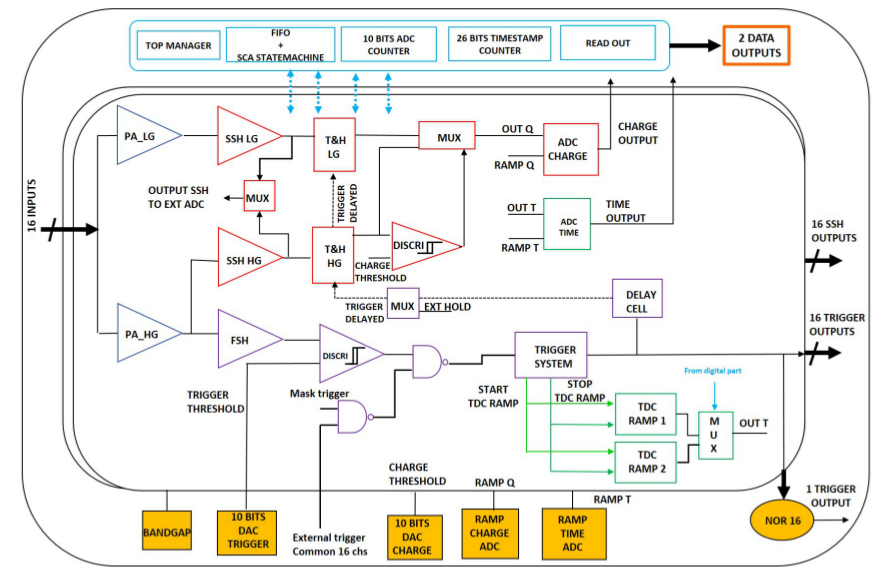
\includegraphics[width=0.7\textwidth]{dpele-lro-catiroc}
\end{dunefigure}

Figure~\ref{fig:dpele-lro-catiroc} shows the schematic of the CatiROC ASIC. Its main properties are summarized in Table~\ref{tab:dpele-catiroc}. The slow channel, from which precision charge and timing measurements are made, is formed by two variable gain (\SI{8}{bit}) amplifiers followed by two variable slow shapers; one High Gain for small signals, and one Low Gain for larger signals, and two Track-and-Hold stages. The slow shaper has a tunable shaping time (up to \SI{100}{ns}) and a variable gain.  If the High Gain is saturated, corresponding to passing a pre-determined threshold common to all 16 channels, the Lower Gain value is chosen. The chosen charge value is converted by an internal 10-bit Wilkinson ADC operating at \SI{160}{MHz}.  This slow channel operates in a ping-pong mode, with two capacitors to store the slow shaper signals, giving an effective buffer of 2 events. If both capacitors are full, a deadtime of \SI{5}{\micro\second} arises.

The fast channel is used to auto-trigger the ASIC and make the fine-timing measurement. It comprises a high gain preamplifier, fast shaper (shaping time \SI{5}{ns}) and discriminator with a \num{10} bit programmable threshold that is common to all \num{16} channels. The output of the discriminator is used for the two Time to Digital Convertors to get the fine-timing. A coarse timestamp could also be obtained from a \num{26} bit counter running at \SI{40}{MHz}.  Only the data from the triggered channels are digitized; their information is transferred to the internal memory, which is read by the external FPGA. 

%Measurements performed in \cite{Blin2017} ..% SNR of 13 trigger efficiency etc...
%total number of bits per channel, 50-bits from CatiROC?
%COPY CAYETANO TABLE
%SELMA'S SPE FROM JUNO?? or my spe??
\begin{dunetable}
[Main characteristics of CatiROC.]
{lr} {tab:dpele-catiroc}
{Main characteristics of CatiROC}
Item &   \\ \toprowrule
Number of channels & \num{16}\\ \colhline
Signal polarity & negative \\ \colhline
Timing & Timestamp: 26 bit counter at \SI{40}{MHz} \\
       & Fine time: resolution $<$\SI{200}{ps}\\ \colhline
Charge Dynamic Range & \SI{160}{\femto\coulomb} to \SI{100}{\pico\coulomb}\\ \colhline
Trigger & auto-trigger \\
        & Noise = \SI{5}{fC} Minimum threshold = \SI{25}{fC} (5$\sigma$)\\ \colhline
Digital & 10-bit Wilkinson ADC at 160 MHz \\ %TWO READOUT AT 80MHZ??
        & Read-out frame of 50 bits \\ \colhline
Outputs & \num{16} trigger outputs \\
        & NOR16 \\
        & \num{16} slow shaper outputs \\
        & Charge measurement over \num{10} bits \\
        & Time measurements over \num{10} bits \\ \colhline
Main Internal &  Variable preamplifier gain \\
Programmable  &  Variable shaping and gain \\
Features & Common trigger threshold \\
         & Common gain threshold \\ \colhline
\end{dunetable}
 
  
%%%%%%%%%%%%%%%%%%%%%%%%%%%%%%%%%%%
\subsection{Network-based uTCA Architecture}
\label{sec:fddp-tpc-elec-design-utca}

The digital electronics is based on uTCA standard which offers industrial solution a very compact and easily scalable architecture to handle a large number of channels at low cost.  The standard (or related standards such as ATCA or xTCA) is widely used in the telecommunication industry and is being adapted by the HEP community. The backplane of the uTCA crates host high-speed serial links that support a variety of transmission protocols (Ethernet, PCI Express, SRIO, etc.). In addition, dedicated lanes are available for the distribution of the clock signals to all the boards hosted in the crate.  The Ethernet-based solution has been adopted for both the data and clock distribution in this design of the DP electronics system for both Charge and Light Read Out. 

Each AMC for either charge or light readout plugged into the uTCA is connected to the crate MCH board through the backplane serial links. The MCH provides the switch functionality that enables AMCs to communicate with each other or external systems through the MCH uplink interface. In the DP electronics system design, MCH also manages the WR clock distribution. 

\begin{dunetable}
[Bandwidth requirements per uTCA crate]
{lr}{tab:dp-utcabandwidth}
{Bandwidth requirements per uTCA crate for continuous data streaming. A compression factor of 10 for the charger readout data is assumed }   
Parameter & Value  \\ \toprowrule
  CRO data rate  &  \SI{1.8}{Gbit/s}         \\ \colhline
  LRO data rate  &  \SI{4.7}{Gbit/s}            \\ \colhline
  Current MCH bandwidth & \SI{10}{Gbit/s}              \\ \colhline
  Upgradable MCH bandwidth & \SI{40}{Gbit/s}           \\ \colhline
\end{dunetable}

In the current design, as used for ProtoDUNE-DP, the MCH operates with a \SI{10}{Gbit/s} uplink. Given that a uTCA crate hosts \num{10} AMCs for charge readout, the required bandwidth to stream the data to DAQ is about \SI{1.8}{Gbit/s}. This assumes that the data exiting the AMCs are losslessly compressed with the compression factor of \num{10}. The bandwidth required per crate link for streaming the light readout data is \SI{4.7}{Gbit/s}. The \SI{10}{Gbit/s} MCH is therefore sufficient to support these data rates. However, the technology is moving towards supporting the \SI{40}{Gbit/s} rates. In addition, the channel density per AMC could also be increased for cost optimization. For these reasons an upgrade to a \SI{40}{Gbit/s} MCH could be foreseen in the future. This would also imply that the optical links connecting the DAQ system to uTCA MCH should be operable at \SI{40}{Gbit/s}. A summary of the required and supported bandwidths per uTCA crate for continous data streaming is provided in Table~\ref{tab:dp-utcabandwidth}.

\begin{dunefigure}[Pictures of an instrumented uTCA crate from LArProto detector]{fig:dpele-311-utca-image}
{Pictures of an instrumented uTCA crate from LArProto detector. The crate contains five AMC cards, correspondingly to the number of readout channels per the SFT chimney. The images below show the crate after the  cables are connected to the warm flange of the SFT chimney.}
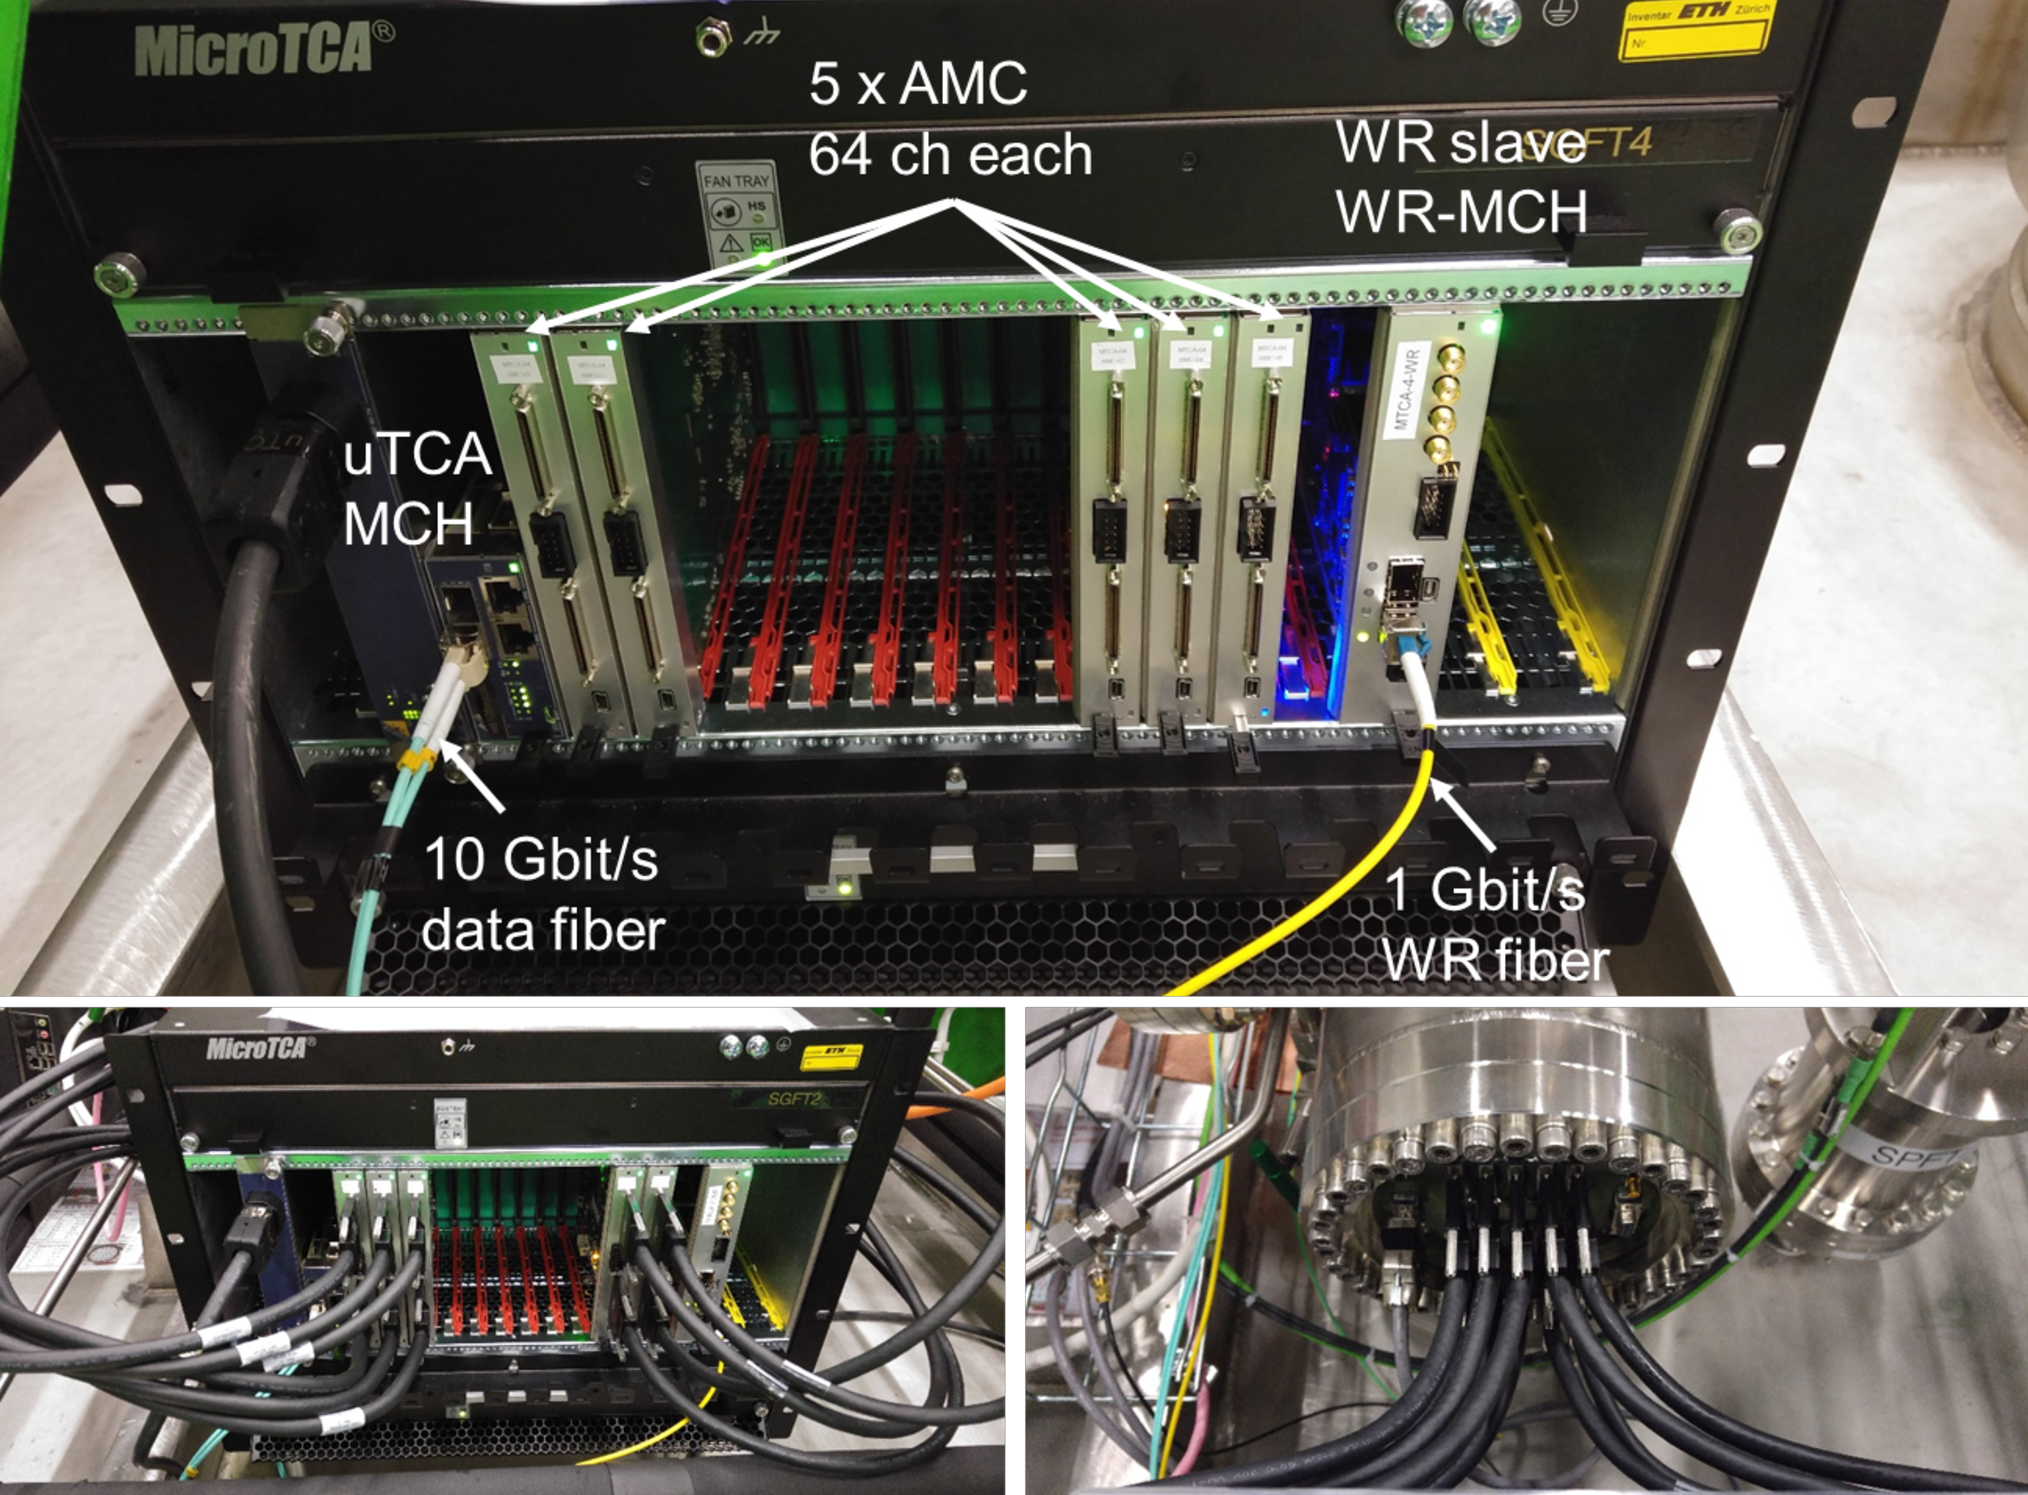
\includegraphics[width=0.6\textwidth]{dpele-311-utca-image}
\end{dunefigure}

As an illustration, Figure~\ref{fig:dpele-311-utca-image} shows pictures of one of the instrumented uTCA crates used for the charge readout of LArProto at CERN. In this detector each SFT chimney reads \num{320} channels thus requiring only five AMCs per the uTCA crate. The two optical fiber links, one (\SI{10}{Gbit/s}) for data and the other (\SI{1}{Gbit/s}) for clock/trigger timing distribution, are visible in the images.       

%%%%%%%%%%%%%%%%%%%%%%%%%%%%%%%%%%%
\subsection{Timing Distribution}
\label{sec:fddp-tpc-elec-wr}
% WR description and card development
The time synchronization system utilizes a White Rabbit (WR) network, which combines the synchronous 1 Gbit/s Ethernet (SyncE) technology with the exchange of PTPV2 packets, to synchronize clocks of distant nodes to a common time. A high stability GPS disciplined oscillator (GPSDO) with the accuracy similar to that of an atomic clock provides a clock reference signal to be distributed over the physical layer interface of the WR Ethernet network. The network topology is built using specially designed switches that have the standard IEE802.1x Ethernet Bridge functionality with an addition of WR-specific extensions to preserve the clock accuracy. Time and frequency information are distributed to the nodes on the WR network via optical fibers. The WR protocol automatically performs dynamic self-calibrations to account for any propagation delays and keeps all connected nodes continuously synchronized to sub-ns precision. 

The sub-ns accuracy on the clock synchronization is not strictly needed for aligning samples in the different AMC digitization units, since the data have the timing granularity of 400 ns. However, WR timing system offers readily available industrial components and necessary protocols needed for synchronization with automatic calibration of delay propagation and it, therefore, has been adopted. The necessary R\&D for integrating this system with the readout of the ProtoDUNE-DP detector has been completed. 

In the implementation specific to ProtoDUNE-DP, a GPS disciplined clock unit (Meinberg LANTIME M600) feeds 10 MHz and 1 PPS reference signals to a commercial White Rabbit switch (Seven Solutions WRS V3.4). The switch acts as Grand Master of the WR network. It is connected via 1Gbit/s optical links to the dedicated WR timestamping node (WR-TSN) and the WR end-node slave cards present within each uTCA crate (WR-MCH) keeping these synchronized to its reference time. The Grand Master also communicates through a standard Ethernet port with the LANTIME unit for its date and time synchronization via NTP. The WR-TSN module recieves analog TTL-level trigger signals, generates their timestamps, and then transmit these over WR network to the connected WR-MCH units. This timestamp information is then used by AMCs to find the data frame corresponding to the trigger. 

\begin{dunefigure}[Picture of White Rabbit slave WR-MCH card]{fig:dpele-wrmch-image}
{Picture of the WR slave node card (WR-MCH) present in each uTCA crate for time synchronization.The WR-LEN mezzanine card is visible in the bottom right corner}
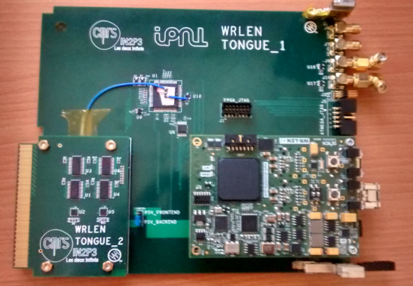
\includegraphics[width=0.45\textwidth]{dpele-wrmch-image}
\end{dunefigure}

The WR-MCH card (Figure~\ref{fig:dpele-wrmch-image}) enables clock/timing/trigger distribution to AMCs. It communicates with them via dedicated lines in the backplane of the uTCA crate using a customized data-frame protocol. The module contains a commercial WR slave node card, the White Rabbit Lite Embedded Node (Seven Solutions OEM WR-LEN), as mezzanine card. WR-LEN runs on a customized firmware which also enables it to decode the trigger timestamp data packet received over the WR network.

\begin{dunefigure}[Architecture of White Rabbit network]{fig:dpele-wrnet-layout}
{Architecture of WR network for time synchronization of digital readout electronics}
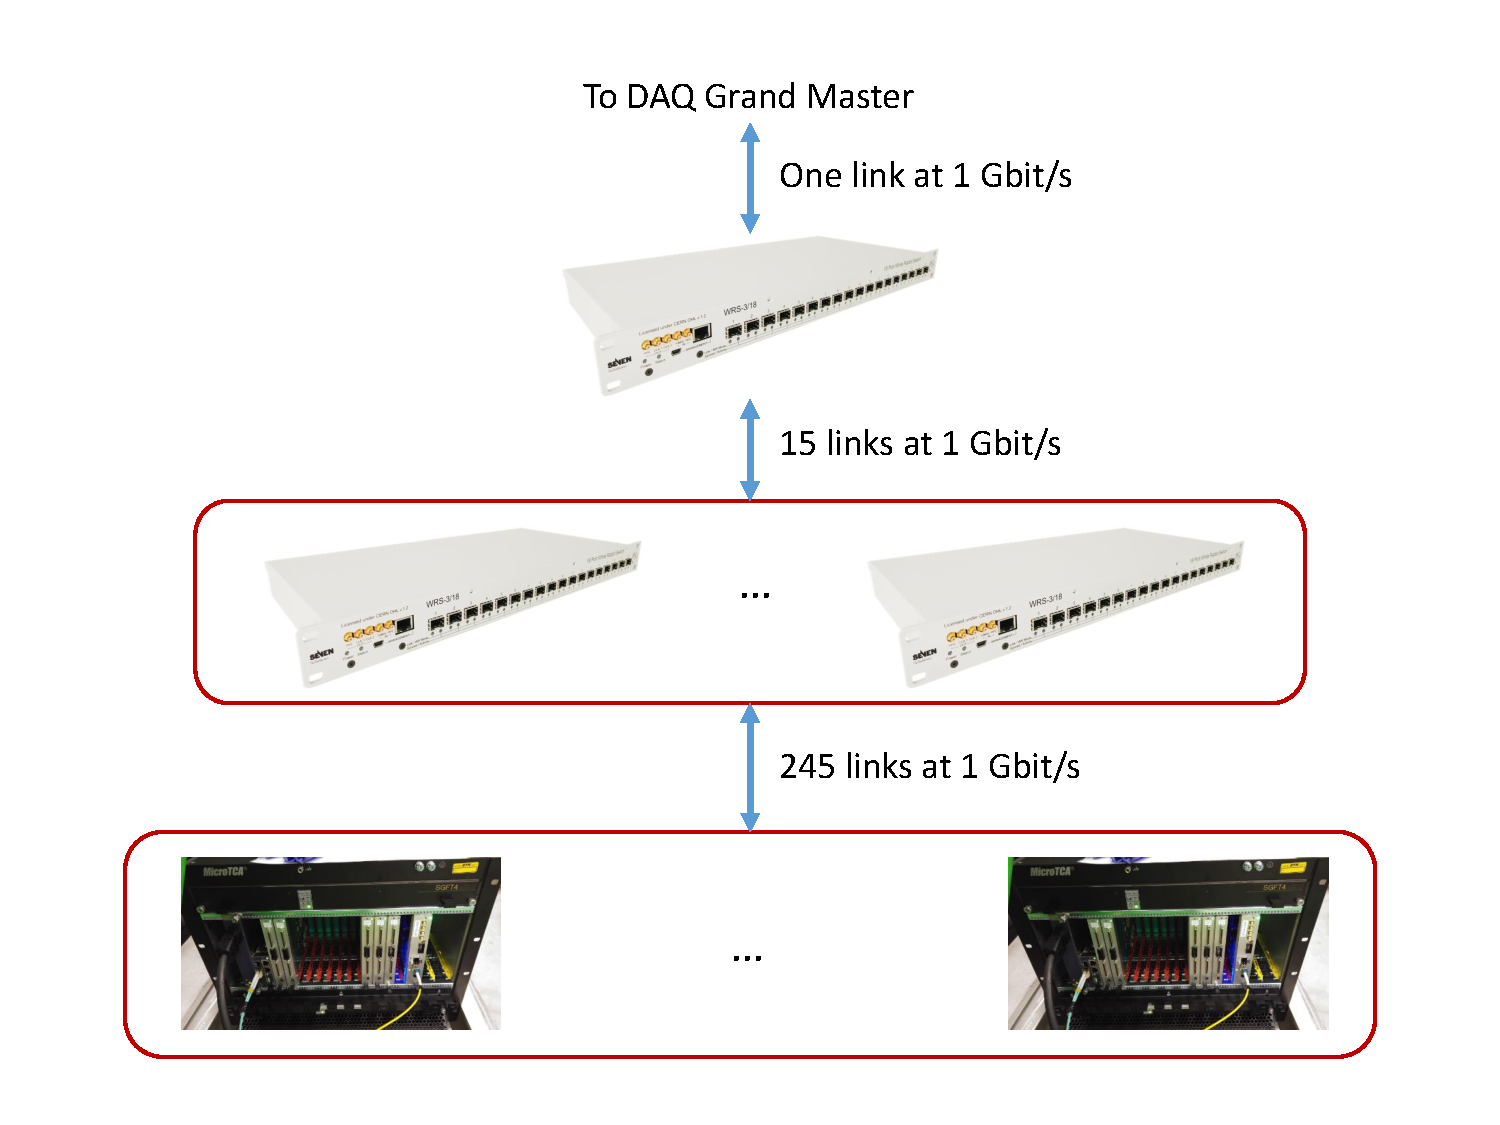
\includegraphics[width=0.7\textwidth]{dpele-wrnet-layout}
\end{dunefigure}

The architecture of the WR network layout for one DP detector module is illustrated Figure~\ref{fig:dpele-wrnet-layout}. It is built in a hierarchical structure from \num{16} WR switches with \num{18} ports each,  chained with \SI{1}{Gbit/s} optical fibers. The switch at the top of the hierarchy interconnects the synchronization Grand Master from the DAQ system with the \num{15} switches in the middle layer. Those are in turn connected to the WR-MCH slave nodes in each uTCA crate (245 in total for charge and light readout). 



%%%%%%%%%%%%%%%%%%%%%%%%%%%%%%%%%%%%%%%%%%%%%%%%%%%%%%%%%%%%%%%%%%%%
\section{Production and Quality Assurance}
\label{sec:fddp-tpc-elec-prod-assy}

%%%%%%%%%%%%%%%%%%%%%%%%%%%%%%%%%%
\subsection{Cryogenic Analog FE Electronics}
\label{sec:fddp-tpc-elec-prod-fe}
The production of the cryogenic ASICs and analog FE cards is envisioned to be split between several sites located in France and Japan at the moment. The delivered cards are then split between between five institutions in France (IPNL), Japan (KEK, NITKC, IU), and USA (SMU), where they are tested. 

%%%%%%%%%%%%%%%%%%%%%%%%%%%%%%%%%%
\subsection{SFT Chimneys}
\label{sec:fddp-tpc-elec-prod-sft}
The production of SFT chimneys consist of manufacturing of the PCB flanges for warm and cold flange interfaces, the stainless steel pipe structure and the flanges containing the interfaces to the gas/liquid lines and slow control, the blades and railing, and the heat exchanger system. The flat cables that connect the FE cards to the warm flange are commercially available products and are also procured at this stage.

The produced pieces are delivered to one or several institutions participating in the DP electronics consortium. The signal continuity is verified for both cold and warm flanges. The SFT chimneys are then assembled and tested for leaks. The blade insertion is also checked and the flat cables are tested. The assembled SFT chimneys are then packed and shipped to SURF. 

%%%%%%%%%%%%%%%%%%%%%%%%%%%%%%%%%%
\subsection{Timing System and uTCA}
\label{sec:fddp-tpc-elec-prod-utca}

The timing system consisting of \num{16} WR switches and the \num{245} uTCA crates containing the power modules, carrier hubs (MCH), and fan units are commercial components. The manufacturer takes the responsibility for the necessary quality control and assurance of these components requiring no further testing on the part of the DP electronics consortium. Once they are delivered to the designated institutions, they can be sent to SURF for the installation. 

The commerical VHDCI signal cables (connecting the AMCs to the SFT chimneys) are procured and tested with the SFT chimney warm flanges.

%%%%%%%%%%%%%%%%%%%%%%%%%%%%%%%%%%
%\subsection{Low-voltage Power Supply System}
%\label{sec:fddp-tpc-elec-prod-lvps}

%%%%%%%%%%%%%%%%%%%%%%%%%%%%%%%%%%%
%\subsection{Digital Electronics}
%\label{sec:fddp-tpc-elec-prod-utca}

\subsection{Charge Readout Electronics}
\label{sec:fddp-tpc-elec-prod-cro}
The production of the AMC cards for the charge readout as well as the WR-MCH slave cards for synchronization is currently shared between four institutions (IPNL, KEK, NITKC, IU). The cards ordered and delivered to each respective institution are subjected to quality assurance tests agreed upon by all participants.  

%%%%%%%%%%%%%%%%%%%%%%%%%%%%%%%%%%%
\subsection{Light Readout Electronics}
\label{sec:fddp-tpc-elec-prod-lro}

The production of the Light Read Out AMC cards is currently envisaged to be made in the same manner as the cards for ProtoDUNE Dual-Phase since the number of cards to be produced, and channels to test, is small. The electronic components will be purchased, to required specifications, for the production of the card. The project will be managed by a qualified engineer, and followed by a specialist in Quality assurance.

The produced cards will be first delivered to the home institutes for testing before being shipped to the DUNE far site.  Basic quality tests will be made upon delivery to ensure conformity of production; including visual inspection and electrical testing.

A series of tests will be performed on each card to ensure their correct fonctionnement and evaluate their performance. Measurements will include; linearity measurements (DNL and INL) of each ADC channel, and tests of the linearity of response of the ASIC. The level of cross-talk on the ASIC must also be quantified.

A dedicated single channel setup, with PMT (Hamamatsu R5912-02-mod), and identical cabling and splitter, can be used to characterise the expected noise level of each channel, and response to single photoelectrons up to saturation. 

Multiple cards will be operated in a uTCA crate with the DUNE DAQ.

After shipping and installation on-site, a small series of tests will be performed with a pulse generator to verify the good working condition of the cards. Noise level measurements will also be made as part of the integration effort.

%%%%%%%%%%%%%%%%%%%%%%%%%%%%%%%%%
%\subsection{Assembly Procedures}
%\label{sec:fddp-tpc-elec-assy}

%%%%%%%%%%%%%%%%%%%%%%%%%%%%%%%%%%%
%\subsection{Quality Assurance}
%\label{sec:fddp-tpc-elec-qa}


%%%%%%%%%%%%%%%%%%%%%%%%%%%%%%%%%%%%%%%%%%%%%%%%%%%%%%%%%%%%%%%%%%%%
\section{Interfaces}
\label{sec:fddp-tpc-elec-intfc}

The DP TPC electronics system has interfaces to several other systems. The system must read the charge and light signals from the detector module and thus needs to interface to CRP and the photo-detection systems.  The digitized data must in turn be transmitted to DAQ via the optical links in each uTCA crate. The SFT chimney need to be integrated in the cryostat structure and connected to the cryogenic/gas  system. The management of the low-voltage power supplies for the FE analog electronics and uTCA crates as well as the monitoring of various sensors in the SFT chimneys have to be part of the slow control. 
Table~\ref{tab:dpele-interfaces} provides the full list of all the relevant interface documents and only some of the principal points are summarized here.

\begin{dunetable}
[Interface documents relevant to DP electronics system]
{lr}{tab:dpele-interfaces}{Interface documents relevant to DP electronics system}   
 FD interface document    & DUNE docdb \\ \toprowrule
DP TPC Electronics to DP CRP & 6751 \\ \colhline
DP TPC Electronics to DP Photon Detector & 6772 \\ \colhline
DP TPC Electronics to Joint DAQ & 6778 \\ \colhline
DP TPC Electronics to Joint CISC & 6784 \\ \colhline
Facility Interfaces to DP TPC Electronics & 6982 \\ \colhline
Installation Interfaces to DP TPC Electronics & 7009 \\ \colhline
Integration Facility to DP TPC Electronics & 7036 \\ \colhline
Calibration to DP TPC Electronics & 7063 \\ \colhline
DUNE Physics to DP TPC Electronics & 7090 \\ \colhline
Software and Computing to DP TPC Electronics & 7117 \\ \colhline
\end{dunetable}

%\fixme{Add in appropriate subsections for the pieces that TPC Electronics interfaces with. These initial ones may not be right.}
\subsection{CRP and Photon Detection System}
\label{sec:fddp-tpc-elec-intfc-crppmt}

The cold flange of the SFT chimneys forms the interface between the CRP and the TPC electronics systems. On the side facing the crystostat the flange hosts \num{20} \num{68} pin connectors (KEL 8930E-068-178MS-F) for plugging the flat cables from the CRP. These are 68 channel twisted pair flat cables each carrying signals from \num{32} anode strips and are part of the CRP system. Each analog FE card reads \num{64} anode strips implying receiving signals from two KEL connectors. The order in which the cables are connected into cold flange determines the mapping of the electronic channels to the physical location of the strips on the CRP and should be coordinated carefully with the CRP consortium. As an illustration, Figure~\ref{fig:dpele-sft-cold-flange} shows some images of the cold flange interface from the LArProto detector.

\begin{dunefigure}[Images of LArProto SFT cold flange]{fig:dpele-sft-cold-flange}
{Images of LArProto SFT cold flange interface with the FE cards inserted (right) and signal cables from CRP connected (left). The LArProto SFT chimneys read only \num{320} channels thus requiring \num{5} FE cards}
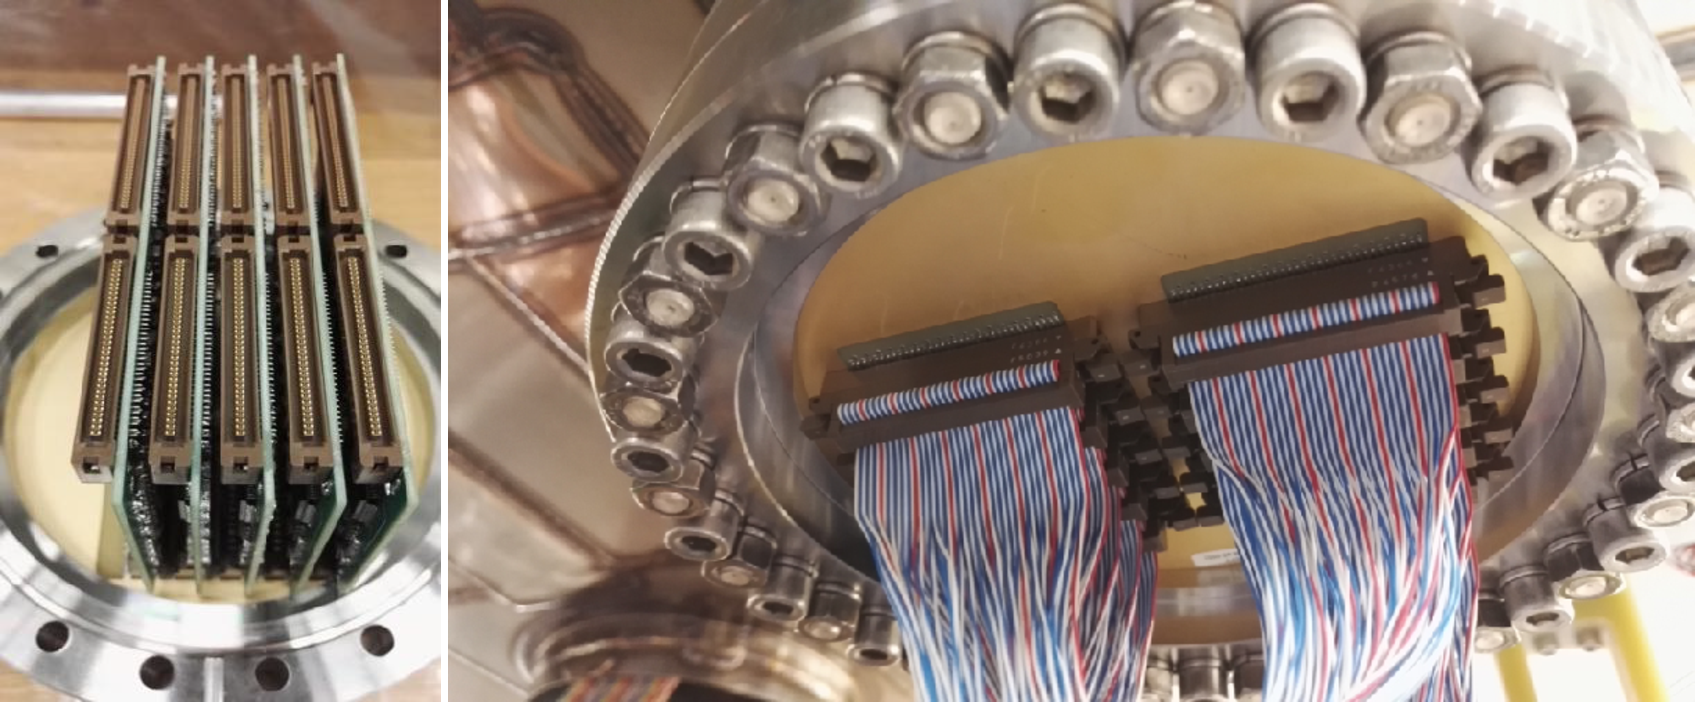
\includegraphics[width=0.8\textwidth]{dpele-sft-cold-flange}
\end{dunefigure}

%\fixme{Interfaces to light readout}
The light readout electronics is designed for negative polarity PMT signals, with the amplitude of single photoelectrons on the input of the card between \num{1} and \SI{10}{\milli\volt}. Typically assuming a PMT gain of \num{1E6} (no accounting for attenuation of the signals), the Catiroc ASIC can measure a range of \num{1} to \num{400} photoelectrons (\SI{160}{\femto\coulomb} to \SI{70}{\pico\coulomb}), the ADC will sample from \SI{1}{\milli\volt} to \SI{1}{\volt} corresponding to \num{1} to \num{1000} photoelectrons, including the time response of the scintillator the range can increase to $\sim$\num{6000}. Increasing the gain of the PMT to \num{1E7}, lowers the upper values by a factor of 10.

The internal noise level of the CatiROC is below \SI{0.1}{\milli\volt}. The objective for the noise level of the ADC is for each channel to have the RMS noise level greater than \SI{0.5}{LSB}, aiming for \SI{1}{LSB} \SI{0.1}{\milli\volt}.
%at 65 MHz...

%%%%%%%%%%%%%%%%%%%%%%%%%%%%%%%%%%%
\subsection{DAQ System}
\label{sec:fddp-tpc-elec-intfc-daq}

The hardware interface between DP-Electronics and DAQ has two components. The first interface is the \SI{10}{Gbit/s} optical fibers for data transfer between the uTCA crates and the network interface of the DAQ system. The second one is a \SI{1}{Gbit/s} optical fiber that connects the DAQ White Rabbit Grand Master switch to the DP electronics timing system.   

In the baseline design a given DP detector module would have \num{245} \SI{10}{Gbit/s} optical links for streaming the digitized data to DAQ from the charge readout (\num{240} links) and light light readout (\num{5} links) electronics housed in uTCA crates on top of the cryostat structure.  In the current specifications, the fibers are multimode OM3 fibers\footnote{http://shop.fiber24.net/index.php/en/FO-Patch-Cable-OM3-Multi-mode-50-125-m-Duplex-LC-PC-LC-PC/c-OM3-DUPLEX-1TO1/a-FOPC-F2-O3-DX-LCU-LCU} with LC-LC connectors suitable for the transmission over distances of up to \SI{300}{\metre}.  They are provided by the DAQ consortium. On the side of the uTCA crate, the fibers are connected to an optical transceiver in the MCH\footnote{http://www.nateurope.com/products/NAT-MCH.html} (two SFP+ (XAUI) links).  On the DAQ, they go to the Level 1 (LV1) machines of the trigger farm, or switches, depending on the network topology adopted in the DAQ system design.

The \SI{1}{Gbit/s} link going from the White Rabbit Grand Master to the DP-electronics time distribution network serves to provide the synchronization to the reference clock common for the entire FD and derived from a GPSDO (GPS-Disciplined Oscillator) clock unit installed on the surface. The clock information is distributed to the WR-MCH slave module in each uTCA crate via a set of White Rabbit switches. These switches and the interconnecting \SI{1}{Gbit/s} fibers form the timing sub-system of the DP electronics system and are included in the design of the latter. The White Rabbit synchronization protocol includes the automatic and continuous calibration of the propagation delays between the master and the connected slaves. This allows maintaining the overall synchronization between different nodes at sub-ns level. The Grand Master could be possibly located 
\begin{itemize}
\item{On surface near to GPSDO. In this case, a single fiber connects it to the DP timing system underground. The incurred latency due to the necessary fiber length to deliver the timing signals underground is automatically taken into account by the system. }
\item{Underground in CUC. In such case, the calibration of the propagation delays between GPSDO and the Grand Master would be performed manually and the timing correction would need be applied to the data afterward.}
\end{itemize} 

The design of the TPC electronics assumes that the data are streamed continuously via the \SI{10}{Gbit/s} links to the DAQ system, where they are buffered until a trigger decision could be made. The triggers are to be issued by processing the buffered data in some suitable sliding time window on the trigger farm machines. The depth of the window may go up to \SI{10}{s} as needed for the definition of the Supernova triggered events. The triggers determine if the data contained in the buffers are to be written on disk. 

The software interface between DAQ and the electronics systems includes the tools dealing with the data transmission and buffering: data formatting in UDP packets, compression/decompression, and exchange of the control packets.

%%%%%%%%%%%%%%%%%%%%%%%%%%%%%%%%%%%
\subsection{Cryostat and Cryogenics}
\label{sec:fddp-tpc-elec-intfc-cryo}

The interface point between the cryostat and the DP electronics system is the cryostat penetrations where the SFT chimneys are to be installed. Each penetration should accommodate the chimney whose external diameter is \SI{254}{\mm}. Each chimney has a CF-273 flange welded to its outer structure (see Figure~\ref{fig:dpele-sft-chimney-crosspipe}). After the chimney is inserted, this flange is in contact with the corresponding flange on the crossing (or penetration) pipe embedded in the cryostat structure to which it is eventually fastened. In order to avoid any leaks at this interface a CF-273 copper gasket is used to ensure the vacuum tightness.  

\begin{dunefigure}[Details of SFT chimney interface to the cryostat structure]{fig:dpele-sft-chimney-crosspipe}
{Details of SFT chimney interface to the cryostat structure}
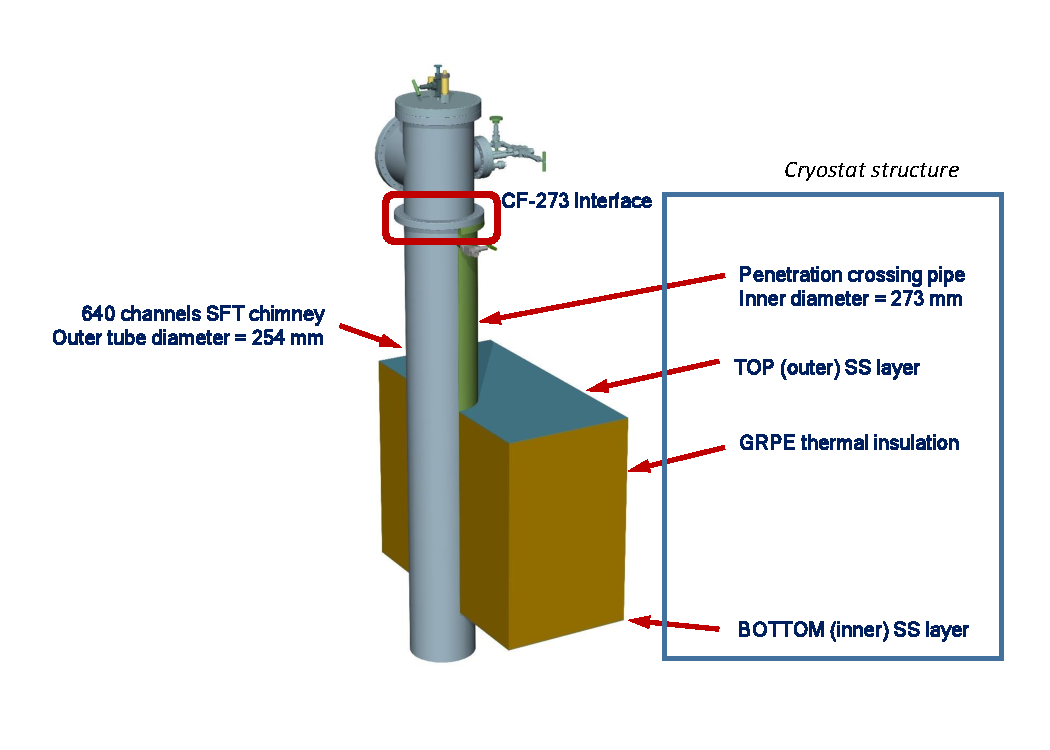
\includegraphics[width=0.7\textwidth]{dpele-sft-chimney-crosspipe}
\end{dunefigure}

Each chimney contains a heat exchanger copper coil cooled with a liquid argon. There are two (inlet/outlet) stainless steel pipe connections with \SI{10}{\mm} (\SI{12}{\mm}) inner (outer) diameter that need to be branched to the respective system for the LAr delivery and re-circulation. In addition, there is a connection for nitrogen gas line with the same pipe dimensions as those for the LAr cooling, which is used for filling the chimney after it is closed following the installation of the FE electronics. The nitrogen line is also required for flushing the chimney in the case of an access to the FE cards after the detector module is cooled for the operation. 

The uTCA crates for charge readout need to be installed within a short \SI{<0.5}{\meter} distance from the SFT chimneys on top of the cryostat roof. The five uTCA crates for the light readout are also placed on the roof of the cryostat at optimal locations defined by the routing of the PMT signal cables. The required volume to accommodate the crates is roughly \SI[product-units=power]{60x50x40}{\cm}. 

%%%%%%%%%%%%%%%%%%%%%%%%%%%%%%%%%%%
\subsection{Slow Control System}
\label{sec:fddp-tpc-elec-intfc-sc}

The integration with the slow control of the low voltage power supply system for the FE cards and uTCA crates is required to enable the remote management and monitoring (current consumption by ASICs, set voltage, etc.). In addition, the SFT chimneys contains several sensors that need to be monitored. These include a pressure transducer that measures the pressure inside the chimney and at least two temperature probes (PT1000) that monitor the gas temperature inside near the cold flange at the bottom and close to the warm flange at the top.  

%%%%%%%%%%%%%%%%%%%%%%%%%%%%%%%%%%%%%%%%%%%%%%%%%%%%%%%%%%%%%%%%%%%%
\section{Installation, Integration and Commissioning}
\label{sec:fddp-tpc-elec-install}

The installation of the TPC electronics systems proceeds in several stages. In order to cable the CRPs to the SFT chimneys, these have to be installed first prior to the start of the CRP installation inside the cryostat. After the chimneys are installed the FE cards could be mounted on the blades and inserted. The installation of the digital electronics and uTCA crates should, however, be postponed until all of the heavy work finishes on top of the cryostat in order to ensure that the fragile components (e.g., optical fibers) are not accidentally damaged due to movement of material and large traffic of personnel. Once the uTCA crates are installed and all the digital cards are inserted, the relevant AMCs are cabled to the warm flanges of the SFTs for the charge readout and are connected to the PMT signal cables for the light readout. Finally to complete the installation and integrate the system with the DAQ, the \SI{10}{Gbit/s} and \SI{1}{Gbit/s} optical links to the DAQ and WR timing network are connected. At this stage the full system is ready for commissioning. 

%%%%%%%%%%%%%%%%%%%%%%%%%%%%%%%%%%%%
\subsection{Transport and Handling}
\label{sec:fddp-tpc-elec-install-transport}
%\fixme{provide rough dimensions for boxes, chimney weights?}
%\fixme{specify that the chimneys are to be delivered for the installation underground and positioned around the cryostat on top.}

The SFT chimneys are \SI{2350}{\mm} long objects with the weight of \SI{180}{\kg}. They are shipped in wooden crates with approximate dimensions of \SI[product-units=power]{2.5x0.5x0.5}{m}. Once on site the crates are moved underground and placed on the roof of the cryostat by the UIT. The personnel from the DP electronics consortium then proceeds to unpack the crates and install the SFT chimneys. The chimneys are delivered with the cold and warm flanges already mounted and after they have been tested for leaks by one or several participating institutions.  

The boxes containing the electronic cards and uTCA crates are handled by DP electronics consortium personnel. These are foreseen to be light and could be easily carried. 

%%%%%%%%%%%%%%%%%%%%%%%%%%%%%%%%%%%
\subsection{SFT Chimneys}
\label{sec:fddp-tpc-elec-install-sft}

The installation of the SFT chimneys requires a compact gantry crane with the supports movable along the length of the cryostat. The crane itself moves along the transverse direction. The crates containing the SFT chimneys are placed along the edges of the cryostat roof. An unpacked chimney is hoisted and transported to its respective penetration crossing pipe for installation. Once in place, the chimney is fastened to the flange on the crossing pipe. The length of each chimney is about \SI{2.4}{m}. Enough overhead room should therefore be foreseen to allow to freely move the chimney with the crane along the direction transverse to the beam axis. 

In parallel with the chimney installation, the FE cards are unpacked and mounted on the blades. This work is performed on the roof of the cryostat to avoid repackaging the blades after the assembly in order to bring them on top of the cryostat. With SFT chimneys secured in the cryostat structure, the blades with mounted FE cards can be inserted and the chimney can be sealed. At this stage, the connections with the pipes for the liquid argon and gas nitrogen delivery could also be made, if these latter have already been installed. The pressure probes and temperature sensors can be connected to the slow control system.
 
%%%%%%%%%%%%%%%%%%%%%%%%%%%%%%%%%%%%
\subsection{Digital uTCA crates}
\label{sec:fddp-tpc-elec-install-utca}
The installation of the uTCA crates with the digital electronics should happen in the final stage of the detector installation to avoid damaging the fragile equipment. The crates are placed in their designated positions on the cryostat and connected to the power distribution network. The AMC cards and WR-MCH modules are inserted in their slots. The VHDCI cables are then attached connecting the CRO AMCs to the warm flange interface of the SFT chimneys.  The fibers from the timing system are connected to WR-MCH. 

%%%%%%%%%%%%%%%%%%%%%%%%%%%%%%%%%%%%
%\subsection{Infrastructure}
%\label{sec:fddp-tpc-elec-install-cable}

%%%%%%%%%%%%%%%%%%%%%%%%%%%%%%%%%%%
%\subsection{Integration}
%\label{sec:fddp-tpc-elec-install-integ}

%%%%%%%%%%%%%%%%%%%%%%%%%%%%%%%%%%%
\subsection{Integration within DAQ}
\label{sec:fddp-tpc-elec-install-daq}
The integration of the DP TPC electronics with the DAQ system requires connecting the \SI{10}{Gbit/s} fiber links to each of \num{245} uTCA crates. The connection of the timing system to the synchronization Grand Master is done via a single \SI{1}{Gbit/s} fiber link. 

The necessary software for the DAQ to read and decode the data packets sent by each uTCA crate would also be provided.   

%%%%%%%%%%%%%%%%%%%%%%%%%%%%%%%%%%%
\subsection{Integration with Photon Detection System}
\label{sec:fddp-tpc-elec-install-pmt}
The cables carrying the PMT signals from the splitter boxes need to be connected to the light readout analog electronics in each uTCA crate. The position of the crates should be optimized with respect to the layout of PMT cables. In addition, the calibration system of the Photon Detection System has to be connected to specified inputs on the cards.

%The light read out cards will recieve the PMT signals via their connection to the splitter boxes. Equally the calibration system of the Photon Detection System will have specified inputs to the cards.
%Anything specific apart from making cable connections? I'm not sure what should go here?

%%%%%%%%%%%%%%%%%%%%%%%%%%%%%%%%%%%
%\subsection{Calibration}
%\label{sec:fddp-tpc-elec-install-calib}

%%%%%%%%%%%%%%%%%%%%%%%%%%%%%%%%%%%
\subsection{Comissioning}
\label{sec:fddp-tpc-elec-install-calib}

The SFT chimneys are commissioned as a first step. The chimneys are evacuated and then filled with nitrogen gas at slight overpressure with respect to the atmospheric pressure.

The electronics system can be commissioned after the installation of the uTCA and the timing system is complete. The functionality of the full DAQ system is not strictly required at this stage. The data from each crate could be read with a portable computer connected to the crate MCH \SI{10}{Gbit/s} or \SI{1}{Gbit/s} interface. By pulsing the CRP strips the non-functioning channels could be identified. The data quality would also be examined to ensure the correct functioning of the digital electronics and the temporal alignment of the data segments.   

%%%%%%%%%%%%%%%%%%%%%%%%%%%%%%%%%%%%%%%%%%%%%%%%%%%%%%%%%%%%%%%%%%%%
%\section{Quality Control}
%\label{sec:fddp-tpc-elec-qc}

%%%%%%%%%%%%%%%%%%%%%%%%%%%%%%%%%%%%
%\subsection{Protection and Assembly (Local)}
%\label{sec:fddp-tpc-elec-qc-local}


%%%%%%%%%%%%%%%%%%%%%%%%%%%%%%%%%%%
%\subsection{Post-factory Installation (Remote)}
%\label{sec:fddp-tpc-elec-qc-remote}


%%%%%%%%%%%%%%%%%%%%%%%%%%%%%%%%%%%%%%%%%%%%%%%%%%%%%%%%%%%%%%%%%%%%
\section{Risks and Vulnerabilities}
\label{sec:fddp-tpc-elec-safety}

The design of the DP electronics system takes into account several risks factors:
\begin{itemize}
\item{\textbf{Obsolescence of electronic components over the period of experiment}: allocation of enough spares (preferably complete cards instead of components) should be sufficient to address this issue. }
\item{\textbf{Modification to FE electronics due to evolution in design of photon detectors}: strict and timely follow-up of the FE requirements from the DP photon system is required.}
\item{\textbf{Damage to electronics due HV discharges or other reasons}: the FE cards should include suitable protection components. The TVS diodes used in the current design have been sufficient to protect the electronics in LArProto detector. In addition, the cards are accessible and could be replaced if damaged. }
\item{\textbf{Overpressure in the SFT chimneys}: the SFT chimneys are equipped with safety valves that vent the excess gas in case of the sudden pressure rise. The overpressure threshold should be set low enough such that no significant damage could happen to the flanges. }
\item{\textbf{Leak of nitrogen inside the detector via cold flange}: the chimney volume would be filled with argon gas instead of nitrogen.}
\item{\textbf{Mechanical problems with FE card extraction due to overhead clearance}: in case of insufficient overhead space it would not be possible to extract the blades from the SFT chimneys. This is addressed by making the requirement for LBNF to ensure there is always enough clearance around the chimneys.}
\item{\textbf{Data flow increase due to inefficient compression caused by higher noise}: currently there is a factor of \num{5} margin in the available bandwidth with \SI{10}{Gbit/s} MCH.}
\item{\textbf{Damage to uTCA crates due to presence of water on the roof of the cryostat}: requirement to LBNF to ensure that the cryostat surface remains dry.}
\item{\textbf{Problems with the ventilation system of the uTCA crates due to bad air quality}: normal conditions similar to any industrial environment at CERN/FNAL should be sufficient to ensure that crates function properly. Liberation of large quantities of dust due to activities in the mine are to be avoided.}
\end{itemize}
%\begin{dunetable}
%[Risks associated with DP electronics system]
%{lr}
%{tab:dpele-risks}{Risks associated with DP electronics system}
%Risk factor  &  Solution \\ \toprowrule
%Obsoleteness of electronic components over the period of experiment & \\ \colhline
%Modification to FE electronics due to evolution in design of photon detectors & \\ \colhline
%Damage to electronics due HV discharges or other reasons & \\ \colhline
%Overpressure in the SFT chimneys & \\ \colhline
%Leak of nitrogen inside the detector via cold flange & \\ \colhline
%Mechanical problems with FE card extraction & \\ \colhline
%Data flow increase due to inefficient compression caused by higher noise & \\ \colhline
%Damage to uTCA crates due to presence of water on the roof of the cryostat & \\ \colhline
%Problems with the ventilation system of the uTCA crates due to bad air quality & \\ \colhline
%\end{dunetable} 


%%%%%%%%%%%%%%%%%%%%%%%%%%%%%%%%%%%
% add subsections and labels if needed \subsection{}
%\label{sec:fddp-tpc-elec-safety-}


%%%%%%%%%%%%%%%%%%%%%%%%%%%%%%%%%%
%\subsection{}
%\label{sec:fddp-tpc-elec-safety}


%%%%%%%%%%%%%%%%%%%%%%%%%%%%%%%%%%%%%%%%%%%%%%%%%%%%%%%%%%%%%%%%%%%%
\section{Organization and Management}
\label{sec:fddp-tpc-elec-org}

%%%%%%%%%%%%%%%%%%%%%%%%%%%%%%%%%%%
\subsection{Dual-Phase TPC Electronics Consortium Organization}
\label{sec:fddp-tpc-elec-org-consortium}

The Dual-Phase TPC electronics consortium actually consists of seven participating institutions from France (\num{3}), Japan (\num{3}), and USA (\num{1}). The consortium leader is Dario Autiero (IPNL, France) and the technical leader is Takuya Hasegawa (KEK, Japan). The composition of the consortium along with the information for each institutional representative is provided in Table~\ref{tab:dpele-consortium-people}.
\begin{dunetable}
[DP TPC electronics consortium current participants]
{p{0.35\linewidth}p{0.25\linewidth}p{0.35\linewidth}}
{tab:dpele-consortium-people}
{DP TPC electronics consortium current participants}   
 Institution    & Investigator & Contact \\ \toprowrule
France: APC  & Thomas Patzak & thomas.patzak@cern.ch \\ \colhline
France: IPNL  & Dario Autiero & autiero@cern.ch  \\ \colhline
France: LAPP & Dominique Duchesneau & duchesneau@lapp.in2p3.fr  \\ \colhline
Japan: Iwate University & Shinya Narita & narita@iwate-u.ac.jp  \\ \colhline
Japan: KEK    & Takuya Hasegawa & takuya.hasegawa@kek \\ \colhline
Japan: NITKC & Seiji Kasai & kasai@kure-nct.ac.jp  \\ \colhline
USA: Southern Methodist University & Thomas Coan & coan@smu.edu  \\ \colhline
\end{dunetable}

%%%%%%%%%%%%%%%%%%%%%%%%%%%%%%%%%%
\subsection{Planning Assumptions}
\label{sec:fddp-tpc-elec-org-assmp}
The present design of the DP TPC electronics system mostly relies on the elements that have already been developed and tested in LArProto detector. Commissioning of the ProtoDUNE-DP towards the end of the year should provide some addition information, but is not expected to affect the design of principal components. Some additional improvements related to the increase in the channel density supported by AMCs  could be envisioned for the purpose of further reduction in costs. 

%%%%%%%%%%%%%%%%%%%%%%%%%%%%%%%%%%%
\subsection{WBS and Responsibilities}
\label{sec:fddp-tpc-elec-org-wbs}

The description of the WBS including the assignments of the responsible institutions is documented in DUNE-doc-5594 and provided in addendum.

%%%%%%%%%%%%%%%%%%%%%%%%%%%%%%%%%%
\subsection{High-level Cost and Schedule}
\label{sec:fddp-tpc-elec-org-cs}

\begin{dunetable}[DP TPC electronics consortium schedule]
{p{0.6\linewidth}lll}
{tab:dpele-schedule}
{DP TPC electronics consortium schedule}
 Techincal activity  &  Days & Start date & End date \\ \toprowrule
Preparation of costing for Technical Proposal & \num{20} & 02/26/18 & 03/23/18 \\ \colhline
Initial Development of Installation Schedule & \num{20} & 02/26/18 & 03/23/18 \\ \colhline
Further Development of Installation Schedule & \num{145} & 09/03/18 & 03/22/19 \\ \colhline
Installation and Commissioning of PD-DP & \num{320} & 01/01/18 & 03/22/19 \\ \colhline
Finalization of the number of channels for light readout & \num{20} & 09/03/18 & 09/28/18 \\ \colhline
Implementation of routing for digital cards of light readout & \num{40} & 10/01/18 & 11/23/18 \\ \colhline
Preparation of final costing for TDR & \num{85} & 11/26/18 & 03/22/19 \\ \colhline
Firmware development for charge readout cards & \num{145} & 09/03/18 & 03/22/19 \\ \colhline
\end{dunetable}

The detailed cost model has been developed based on the scaling of the costs for the electronics system of ProtoDUNE-DP. It is provided in addendum. 
Table~\ref{tab:dpele-schedule} shows an extract from the international project schedule pertaining to the technical activities of the consortium.



